\newpage
\section{Bijlage 1.}
\label{b1}


\subsection{Bevolkingsgroep: Allochtonen.}
\label{allochtonen}

Betreffende de bevolkingsgroep allochtonen in Nederland worden hieronder de resultaten van de verschillende strategie\"{e}n uiteengezet om zodoende te achterhalen met welke strategie in theorie de meeste allochtone kandidaten in de Tweede Kamer gekozen kunnen worden wanneer alle stemgerechtigde allochtone kiezers in Nederland zich committeren aan de strategie.\\
\indent In deze sectie worden enkel strategie 1 en strategie 2 toegepast. Strategie 3.1, strategie 3.2 en strategie 4 worden op de bevolkingsgroep allochtonen niet toegepast omdat er te weinig allochtonen op de kandidatenlijsten staan om op de top 15 allochtone kandidaten te stemmen (strategie 3.1) en om voor elke partij een eigen top \textit{N} vast te stellen op basis van aantal allochtone kandidaten (strategie 3.2). Tevens hebben de partijen waar meer allochtone kandidaten op de kandidatenlijst staan dan dat deze partijen aan zetels konden gaan verwachten, te weinig allochtone stemmen ontvangen om een extra percentage aan zetels (voor allochtone kandidaten) bij de \textit{N} toe te voegen (strategie 4).\\
\indent Ten behoeve van de leesbaarheid worden er geen voorbeelden gegeven betreffende berekeningen. Alle voorbeelden zijn te vertalen vanuit de bij de bevolkingsgroep vrouwen toegepaste strategie\"{e}n (zie Sectie \ref{vrouwen}). 

\paragraph{Aannames en Regels.}
De aannames en regels zijn hetzelfde als bij de strategie\"{e}n voor de bevolkingsgroep vrouwen . Hierbij moet genoteerd worden dat vrouwen vervangen dient te worden voor allochtonen en vrouwelijke kandidaten vervangen dient te worden voor allochtone kandidaten (voor een gedetailleerde omschrijving van de aannames zie Sectie \hyperref[besS]{Beschrijving Strategie\"{e}n} en voor de regels van een strategie zie correspondeerde strategie in Sectie \ref{vrouwen}).

\paragraph{Het berekenen van het aantal te verwachten allochtone stemmen.}
\iffalse
Eerder in dit hoofdstuk wordt er in detail aan de hand van enkele voorbeelden uitgelegd hoe het aantal te verwachten vrouwelijke stemmen kan worden berekend (zie Sectie \hyperref[vrouwen]{Bevolkingsgroep: Vrouwen}). In deze sectie wordt de bevolkingsgroep allochtonen in Nederland behandeld. De manier van berekenen is hetzelfde bij de deze bevolkingsgroep als bij de bevolkingsgroep vrouwen in Nederland. 
\fi
Op 1 september 2012 waren er 2.629.699 allochtonen boven de 18 jaar wonenden in Nederland \citep{CBS_allochtonen}. We gaan er voor deze bevolkingsgroep vanuit dat al deze personen stemgerechtigd waren tijdens de Tweede Kamerverkiezingen van 2012. De peiling onder allochtonen \citep{Opiniehuis} gaf aan dat 55\% van de allochtonen zou gaan stemmen. Dat komt neer op (55\%*2.629.699 = ) 1.446.334 stemmen. Op een vergelijkbare wijze als bij de bevolkingsgroep vrouwen, is voor de bevolkingsgroep allochtonen berekend hoeveel stemmen de partijen van allochtone kiezers konden gaan verwachten. Hierbij is het allochtoon stempercentage het percentage van alle door allochtonen uitgebrachte stemmen. Ter illustratie nemen we GROENLINKS als voorbeeld. \\
\indent Volgens de peiling zou GROENLINKS 2,1\% van de allochtone stemmen krijgen. Zoals eerder al berekend, is het aantal stemgerechtigde allochtonen dat gaat stemmen een aantal van 1.446.334. Daarmee komt GROENLINKS op een aantal van ($2,1\%*1.446.334$ = ) 30.373 allochtone stemmen. In Tabel \ref{table:tab1A} hieronder is per partij het allochtone stempercentage te zien evenals het aantal stemmen de partij zou gaan ontvangen van allochtone kiezers.  

\begin{table}[H]
\centering
	\begin{footnotesize}
		\begin{tabular}{lrr}
\toprule
 &  Allochtone Stempercentage  &  Aantal Stemmen Van Allochtonen \\
Partij                &                        &                                 \\
\midrule
50PLUS                &                 0,0 &                               0 \\
CDA                   &                 2,1 &                           30.373 \\
ChristenUnie          &                 0,2 &                            2.893 \\
D66                   &                 7,6 &                          109.921 \\
GROENLINKS            &                 2,5 &                           36.158 \\
Partij v d Dieren &                 0,6 &                            8.678 \\
PVDA                  &                40,9 &                          591.551 \\
PVV                   &                4,7 &                           67.978 \\
SGP                   &                 0,0 &                               0 \\
SP                    &                19,1 &                          276.250 \\
VVD                   &                4,7 &                           67.978 \\
Weet Niet		      & 				17,6 & 						254.555 \\
\midrule
Totaal				&					100	&						1.446.334\\
\bottomrule
\end{tabular}

	\end{footnotesize}
			\caption{Het allochtone stempercentage en het totaal aantal te verwachten allochtone stemmen volgens de peiling.}
\label{table:tab1A} 
\end{table}


\paragraph{Het berekenen van het daadwerkelijke aantal allochtone stemmen.}
\iffalse
Eerder in dit hoofdstuk wordt er in detail aan de hand van enkele voorbeelden uitgelegd hoe het daadwerkelijke aantal vrouwelijke stemmen kan worden berekend (zie Sectie \hyperref[vrouwen]{Bevolkingsgroep: Vrouwen}). Ook hier is de manier van berekenen van het daadwerkelijke aantal allochtone stemmen hetzelfde als bij de bevolkingsgroep vrouwen.
\fi
De opkomst onder allochtonen lag aanzienlijk hoger dan de peiling van Opiniehuis \citeyearpar{Opiniehuis} had aangegeven met 55\% volgens de peiling om 66\% volgens het CBS \citeyearpar{CBS_stemgedrag}. Er zijn dus meer stemmen door allochtonen uitgebracht dan werd verwacht. Het aantal uitgebrachte allochtone stemmen komt hiermee op ($66\%*2.629.699$ = ) 1.736.055 stemmen. Daarnaast zat de peiling van Opiniehuis er bij een aantal partijen flink naast.  Hieronder is in Tabel \ref{table:tab2A} per partij te zien hoeveel procent van de allochtonen kiezers op de partij heeft gestemd en het aantal stemmen dat een partij van allochtonen heeft ontvangen. Op dezelfde wijze als het berekenen van het aantal te verwachten allochtone stemmen in de vorige paragraaf, is ook het daadwerkelijke aantal allochtone stemmen per partij berekend.
    
\begin{table}[h]
\centering
	\begin{footnotesize}
		\begin{tabular}{lrr}
\toprule
{} &  Allochtone Stempercentage &  Aantal Allochtone Stemmen \\
Partij                &                            &                            \\
\midrule
50PLUS                &                       1,27 &                      22045 \\
CDA                   &                       3,80 &                      65963 \\
ChristenUnie          &                       3,05 &                      52944 \\
D66                   &                       8,32 &                     144425 \\
GROENLINKS            &                       2,30 &                      39925 \\
Partij voor de Dieren &                       1,27 &                      22045 \\
PVDA                  &                      40,83 &                     708936 \\
PVV                   &                       8,31 &                     144252 \\
SGP                   &                       1,27 &                      22045 \\
SP                    &                       9,09 &                     157792 \\
VVD                   &                      20,49 &                     355683 \\
\midrule
Totaal				& 						100 & 			1736055 \\
\bottomrule
\end{tabular}



	\end{footnotesize}
			\caption{Totaal aantal stemmen dat een partij heeft ontvangen, het aandeel stemmen van allochtonen in percentage en het totaal aantal vrouwelijke stemmen volgens de einduitslag.}
\label{table:tab2A} 
\end{table}
    
\newpage
\subsubsection{Strategie 1: Allochtone kiezers stemmen op top \textit{N} allochtone kandidaten.} \label{S1A}



\paragraph{Verdelingen zetels en aantal allochtone kandidaten.}
In de grafiek hieronder in Figuur \ref{fig:zetelsA} is te zien dat voor alle partijen links van de stippellijn de top \textit{N} gelijk is aan het aantal allochtonen dat de partij op de kandidatenlijst had staan. Bij de partijen rechts van de stippellijn is \textit{N} gelijk aan het aantal te verwachten zetels volgens de peiling. 
 
\begin{figure}[H]

	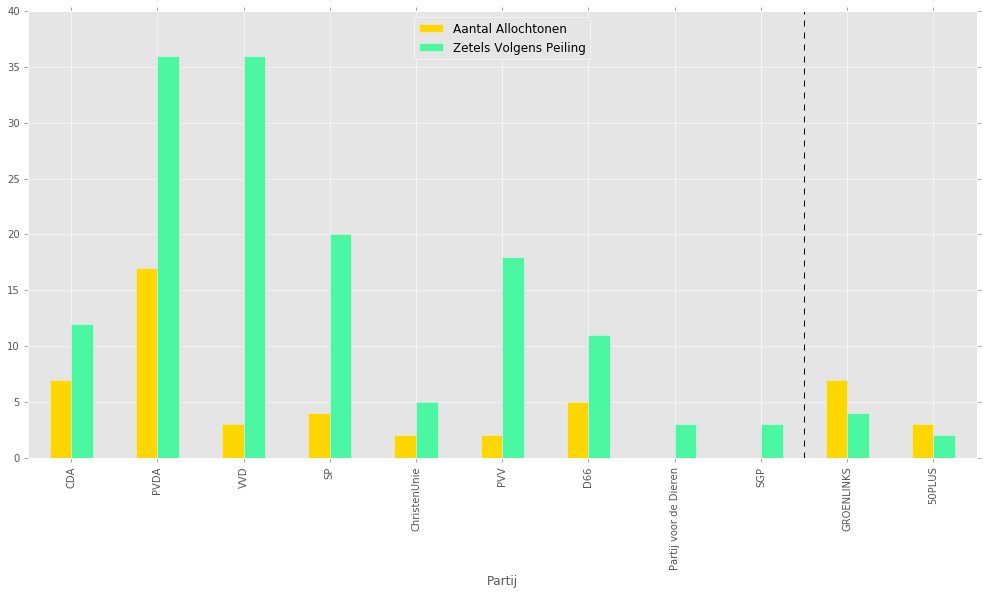
\includegraphics[width=\linewidth]	{Aantal_allochtonen_aantal_zetels.png}

			\caption{Het aantal allochtonen op de kandidatenlijst(geel) en het aantal zetels volgens de peilingen(groen) per partij.}

\label{fig:zetelsA}
\end{figure}


\paragraph{Maximaal aantal allochtonen per partij(top \textit{N}) dat in de Tweede Kamer gekozen kan worden.}
In Tabel \ref{table:tab3A} hieronder is, in het verlengde van Figuur \ref{fig:zetelsA} hierboven, te zien hoeveel allochtone kandidaten er per partij maximaal in de Tweede Kamer gekozen hadden kunnen worden. In de Tabel is dus per partij het aantal (\textit{N}) allochtone kandidaten te zien waarover de stemmen van de allochtone kiezers op de partij verdeeld zullen worden.  
\\
\indent Vanwege het feit dat de SGP en de Partij voor de Dieren helemaal geen allochtone kandidaten op de kandidatenlijst hadden staan en alle partijen, op GROENLINKS en 50PLUS na, meer zetels zullen gaan ontvangen dan dat zij allochtone kandidaten op de kandidatenlijsten hebben staan komt het totaal aantal allochtone kandidaten dat volgens de peiling in de Tweede Kamer gekozen kan worden uit op 46. 





\begin{table}[H]
\centering
	\begin{footnotesize}
		\begin{tabular}{lrr}
\toprule
{} &  Top N Allochtone Kandidaten &  Overgebleven Autochtone Kandidaten \\
Partij                &                              &                                     \\
\midrule
50PLUS                &                            2 &                                   0 \\
CDA                   &                            7 &                                   5 \\
ChristenUnie          &                            2 &                                   3 \\
D66                   &                            5 &                                   6 \\
GROENLINKS            &                            4 &                                   0 \\
Partij voor de Dieren &                            0 &                                   3 \\
PVDA                  &                           17 &                                  19 \\
PVV                   &                            2 &                                  16 \\
SGP                   &                            0 &                                   3 \\
SP                    &                            4 &                                  16 \\
VVD                   &                            3 &                                  33 \\
\midrule
Totaal                &                           46 &                                 104 \\
\bottomrule
\end{tabular}

	\end{footnotesize}
			\caption{Per partij de top \textit{N} allochtone kandidaten en de overgebleven autochtone kandidaten a.d.h.v. de peiling.}
\label{table:tab3A} 
\end{table}



\paragraph{Het toewijzen van de stemmen aan de allochtone kandidaten op basis van de peiling en de einduitslag.}
Op dezelfde wijze als bij de andere strategie\"{e}n wijzen we de hier de allochtone stemmen toe a.d.h.v. de peiling en a.d.h.v. de einduitslag (voor gedetailleerde uitleg zie \hyperref[S1V]{Strategie 1}in \hyperref[vrouwen]{Bevolkingsgroep: Vrouwen}). In Figuur \ref{fig:stemmenS1A} hieronder is zowel de toewijzing op basis van de peiling alsmede de toewijzing op basis van de einduitslag te zien.





\begin{figure}[H]

	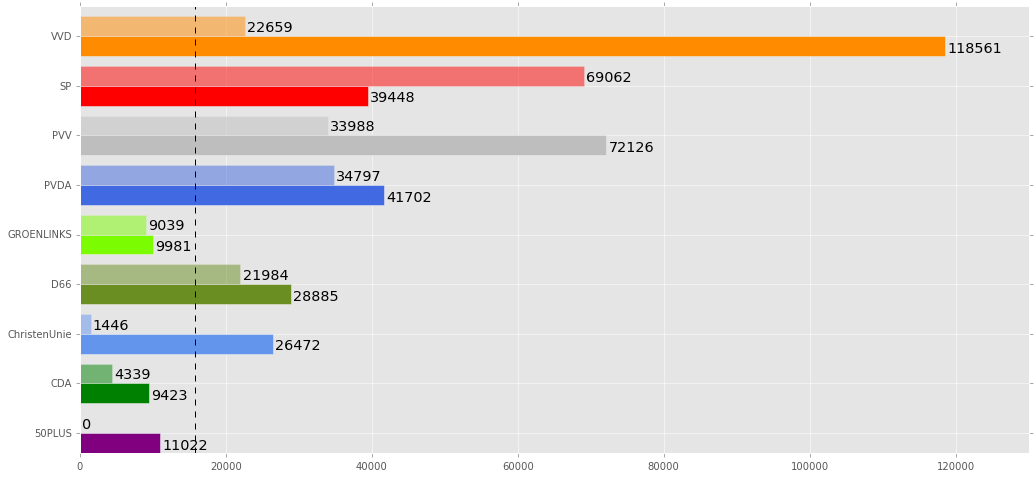
\includegraphics[width=\linewidth]	{stemmen_op_allochtonen_topN_samen2.png}

			\caption{Grafiek met per partij de verdeling van de stemmen van allochtone kiezers op alle vrouwelijke kandidaten van de partij a.d.h.v. de peiling (licht gekleurd) en a.d.h.v. de einduitslag (donker gekleurd) na strategie 1. De stippellijn is de daadwerkelijk voorkeursdrempel(15.708 stemmen).}

\label{fig:stemmenS1A}
\end{figure}


Zoals te zien in Figuur \ref{fig:stemmenS1A} hierboven, zijn bij het toewijzen van de stemmen er enige inconsistenties tussen de voorspelling op basis van de peiling en de einduitslag. Dit kom voornamelijk vanwege het feit dat de peiling onder allochtonen van het Opiniehuis (bron) flink afweek van de werkelijkheid. Echter is de voorspelling a.d.h.v. de peiling grotendeels correct in het voorspellen van welke partijen de allochtone kandidaten boven de voorkeursdrempel komen. Alleen wat betreft de ChristenUnie was de voorspelling niet toereikend.

\paragraph{Aantal allochtonen na strategie 1.}
Na het uitvoeren van de strategie 1 en het opstellen van de Tweede Kamer zoals eerder in dit hoofdstuk beschreven, levert strategie 1 een Tweede Kamer op waarin 34 allochtonen en 116 autochtonen plaatsnemen. Daarmee zijn allochtonen ruim in betere mate vertegenwoordigd dan daadwerkelijk bij de einduitslag van 2012 (dertien zetels bij einduitslag van 2012) het geval was. In de cirkeldiagram in Figuur \ref{fig:pcS1A} hieronder is de verdeling goed te zien. 

\begin{figure}[H]
\centering
	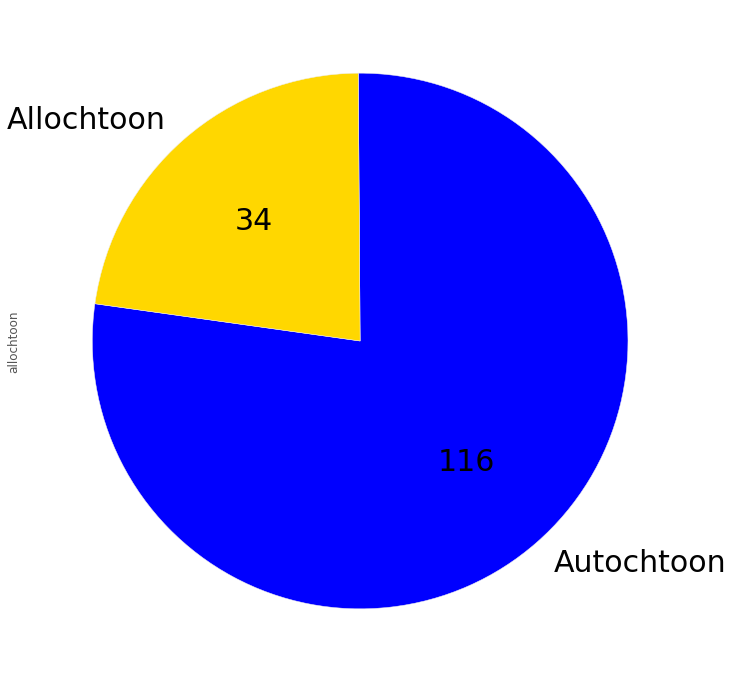
\includegraphics[width=0.35\linewidth]{pie_chart_topN_allochtonen.png}

			\caption{Na uitvoering van de strategie nemen er 34 allochtonen(23\%) en 116 autochtonen(77\%) plaats in de Tweede Kamer.} 

\label{fig:pcS1A}
\end{figure}

\paragraph{Minder vrouwen dan 46 allochtonen in de Tweede Kamer na uitvoering van strategie 1.}
De reden dat er niet 46 vrouwen maar 'slechts' 34 allochtonen in de Tweede Kamer plaatsnemen na uitvoering van strategie 1 ligt ten grondslag aan een aantal factoren. Bij de ChristenUnie, D66, de PVDA, de PVV, de SP en de VVD zijn alle allochtone kandidaten boven de voorkeursdrempel gekomen en hebben daarmee een zetel verkregen. Deze partijen samen zijn goed voor 33 door allochtonen verkregen zetels. De andere partijen had niet genoeg allochtone stemmen ontvangen om de top \textit{N} allochtone kandidaten boven de voorkeursdrempel te helpen. Hierdoor vallen er in totaal 12 allochtone kandidaten af. Echter had GROENLINKS, in de persoon van Jesse Klaver, toevallig een allochtone kandidaat die vanwege zijn plaatst op de kandidatenlijst toch een zetels heeft gekregen.
Het totaal aantal allochtonen in de Tweede Kamer na uitvoering van strategie 1 komt daarom uit op ($46-12$ = ) 34. 


\subsubsection{Strategie 2: Allochtone kiezers stemmen op een willekeurige vrouwelijke kandidaat.}





\paragraph{Het toewijzen van de stemmen aan de allochtone kandidaten op basis van de peiling en de einduitslag.}
Op dezelfde wijze als bij de andere strategie\"{e}n wijzen we de hier de allochtone stemmen toe a.d.h.v. de peiling en a.d.h.v. de einduitslag (voor gedetailleerde uitleg zie \hyperref[S1V]{Strategie 1 }in \hyperref[vrouwen]{Bevolkingsgroep: Vrouwen}). In Figuur \ref{fig:stemmenS2A} hieronder is zowel de toewijzing op basis van de peiling alsmede de toewijzing op basis van de einduitslag te zien.
 


\begin{figure}[H]

	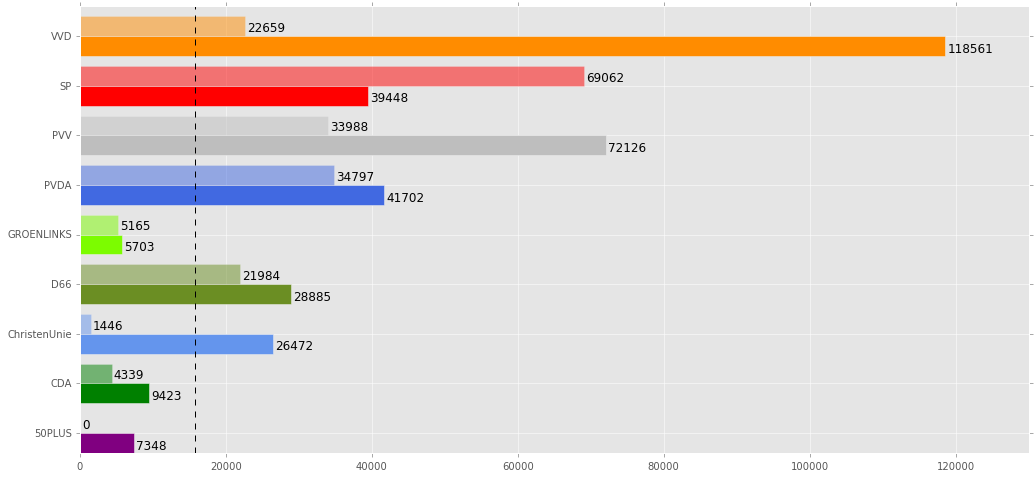
\includegraphics[width=\linewidth]	{stemmen_op_allochtonen_willekeurig_samen2.png}

			\caption{Grafiek met per partij de verdeling van de stemmen van allochtone kiezers op alle vrouwelijke kandidaten van de partij a.d.h.v. de peiling (licht gekleurd) en a.d.h.v. de einduitslag (donker gekleurd). De stippellijn is de daadwerkelijk voorkeursdrempel(15.708 stemmen).}

\label{fig:stemmenS2A}
\end{figure}

Net zoals bij strategie 1 het geval was en zoals te zien in Figuur \ref{fig:stemmenS2A} hierboven, zijn bij het toewijzen van de stemmen er enige inconsistenties tussen de voorspelling op basis van de peiling en de einduitslag (Zie \hyperref[S1A]{strategie 1} in Sectie \ref{allochtonen} voor verklaring).

\paragraph{Aantal allochtonen na strategie 2.}
Na het uitvoeren van de strategie 2 en het opstellen van de Tweede Kamer zoals eerder in dit hoofdstuk beschreven, levert strategie 2 een Tweede Kamer op waarin 34 allochtonen (23\%) en 116 autochtonen (77\%) plaatsnemen. Daarmee zijn allochtonen ruim in betere mate vertegenwoordigd dan daadwerkelijk bij de einduitslag van 2012 (dertien zetels bij einduitslag van 2012) het geval was. In de cirkeldiagram in Figuur \ref{fig:pcS2A} hieronder is de verdeling goed te zien. 


\begin{figure}[H]
\centering
	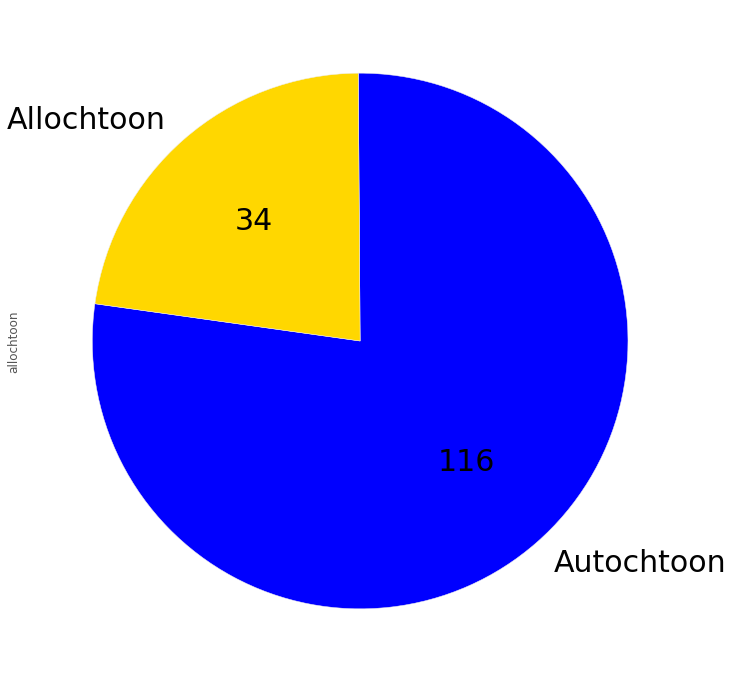
\includegraphics[width=0.35\linewidth]{pie_chart_topN_allochtonen.png}

			\caption{Na uitvoering van de strategie nemen er 34 allochtonen(23\%) en 116 autochtonen(77\%) plaats in de Tweede Kamer.}

\label{fig:pcS2A}
\end{figure}





\paragraph{Hetzelfde aantal allochtonen in de Tweede Kamer als bij strategie 1.}
De reden dat er precies hetzelfde aantal allochtonen in de Tweede Kamer worden gekozen bij strategie 2 ten opzicht van strategie 1 ligt ten grondslag aan een aantal factoren. Zoals het geval is bij strategie 1, zijn bij de ChristenUnie, D66, de PVDA, de PVV, de SP en de VVD alle allochtone kandidaten boven de voorkeursdrempel uitgekomen en hebben zij daarmee een zetel gekregen. Dit komt neer op een aantal van 33 door allochtonen verkregen zetels. Daarnaast hebben de overige partijen, net als bij strategie 1, niet genoeg allochtone stemmen ontvangen om de allochtone kandidaten boven de voorkeursdrempel te helpen. De 34e zetel voor een allochtoon was, net als bij strategie 1, Jesse Klaver. Echter heeft hij een zetels verkregen op basis van zijn plaats op de kandidatenlijst. 



\subsection{Bevolkingsgroep: Ouderen.} \label{ouderen}

Betreffende de bevolkingsgroep ouderen in Nederland worden hieronder de resultaten van de verschillende strategie\"{e}n uiteengezet om zodoende te achterhalen met welke strategie in theorie de meeste oudere kandidaten in de Tweede Kamer gekozen kunnen worden wanneer alle stemgerechtigde ouderen kiezers in Nederland zich committeren aan de strategie.\\
\indent Ten behoeve van de leesbaarheid worden er geen voorbeelden gegeven betreffende berekeningen. Alle voorbeelden zijn te vertalen vanuit de bij de bevolkingsgroep vrouwen toegepaste strategie\"{e}n (zie Sectie \ref{vrouwen}). 

\paragraph{Aannames en Regels.}
De aannames en regels zijn hetzelfde als bij de strategie\"{e}n voor de bevolkingsgroep vrouwen . Hierbij moet genoteerd worden dat vrouwen vervangen dient te worden voor ouderen en vrouwelijke kandidaten vervangen dient te worden voor oudere kandidaten (voor een gedetailleerde omschrijving van de aannames zie Sectie \hyperref[besS]{Bescrijving Strategie\"{e}n} en voor de regels van een strategie zie correspondeerde strategie in Sectie \ref{vrouwen}).

\paragraph{Het berekenen van het aantal te verwachten ouderen stemmen.}
\iffalse
Eerder in dit hoofdstuk wordt er in detail aan de hand van enkele voorbeelden uitgelegd hoe het aantal te verwachten vrouwelijke stemmen kan worden berekend (zie Sectie \hyperref[vrouwen]{Bevolkingsgroep: Vrouwen}). In deze sectie wordt de bevolkingsgroep ouderen in Nederland behandeld. De manier van berekenen is hetzelfde bij de deze bevolkingsgroep als bij de bevolkingsgroep vrouwen in Nederland. 
\fi
Op 1 september 2012 waren er 6.189.591 ouderen (boven de 50 jaar) wonenden in Nederland(CBS, 2012). We gaan er voor deze bevolkingsgroep vanuit dat al deze personen stemgerechtigd waren tijdens de Tweede Kamerverkiezingen van 2012. Vanwege het ontbreken van een peiling onder de oudere kiezers nemen we aan dat de ouderen kiezers hetzelfde stemgedrag vertonen als de Nederlandse kiezers vertoonden volgens de landelijke peiling. We gaan derhalve uit van een opkomst van 73\% (zoals de landelijke peiling aangaf). Dat komt neer op een aantal van (73\%*6.189.591 = ) 4.518.401 stemmen. Op dezelfde wijze als bij de bevolkingsgroep allochtonen, is voor de bevolkingsgroep ouderen berekend hoeveel stemmen de partijen van oudere kiezers konden gaan verwachten (zie Sectie \ref{allochtonen} voor uitleg) . In Tabel \ref{table:tab1O} hieronder is per partij te zien hoeveel procent van de oudere kiezers op een partij heeft gestemd en het aantal stemmen dat een partij van ouderen heeft ontvangen.


\begin{table}[H]
\centering
	\begin{footnotesize}
		\begin{tabular}{lrr}
\toprule
{} &  Oudere Stempercentage &  Aantal Stemmen Van Ouderen \\
Partij                &                        &                             \\
\midrule
50PLUS                &                   1,33 &                       60245 \\
CDA                   &                   8,00 &                      361472 \\
ChristenUnie          &                   3,33 &                      150613 \\
D66                   &                   7,33 &                      331349 \\
GROENLINKS            &                   2,67 &                      120490 \\
Partij voor de Dieren &                   2,00 &                       90368 \\
PVDA                  &                  24,00 &                     1084416 \\
PVV                   &                  12,00 &                      542208 \\
SGP                   &                   2,00 &                       90368 \\
SP                    &                  13,34 &                      602456 \\
VVD                   &                  24,00 &                     1084416 \\
\midrule
Totaal				&				100		&						4.518.401\\
\bottomrule
\end{tabular}

	\end{footnotesize}
			\caption{Totaal aantal stemmen dat een partij zou gaan ontvangen en het totaal aantal te verwachten oudere stemmen volgens de peiling.}
\label{table:tab1O} 
\end{table}


\paragraph{Het berekenen van het daadwerkelijke aantal oudere stemmen.}
\iffalse
Eerder in dit hoofdstuk wordt er in detail aan de hand van enkele voorbeelden uitgelegd hoe het daadwerkelijke aantal vrouwelijke stemmen kan worden berekend (zie Sectie \hyperref[vrouwen]{Bevolkingsgroep: Vrouwen}). Ook hier is de manier van berekenen van het daadwerkelijke aantal oudere stemmen hetzelfde als bij de bevolkingsgroep vrouwen.
\fi 
Vanwege het ontbreken een peiling onder ouderen was er ook geen prognose over de verwachte opkomst. Daarom hebben we de landelijke opkomstprognose van 73\% genomen. Echter was er een opkomst van 75\% onder de ouderen (CBS). Het aantal uitgebrachte oudere stemmen komt hiermee op ($75\%*6.189.591$ = ) 4.642.193 stemmen. Hieronder in Tabel \ref{table:tab2O} is per partij te zien hoeveel procent van de oudere kiezers op de partij heeft gestemd en het aantal stemmen dat een partij van ouderen heeft ontvangen. Op dezelfde wijze als het berekenen aantal te verwachten allochtone stemmen (zie \hyperref[S1A]{strategie 1} in Sectie \ref{allochtonen}), is ook het daadwerkelijk aantal oudere stemmen per partij berekend. 
    
\begin{table}[h]
\centering
	\begin{footnotesize}
		\begin{tabular}{lrr}
\toprule
{} &  Ouderen Stempercentage &  Aantal Ouderen Stemmen \\
Partij                &                         &                         \\
\midrule
50PLUS                &                    4,00 &                  185687 \\
CDA                   &                    8,00 &                  371375 \\
ChristenUnie          &                    2,67 &                  123792 \\
D66                   &                    8,00 &                  371375 \\
GROENLINKS            &                    2,67 &                  123792 \\
Partij v d Dieren &                    1,33 &                   61895 \\
PVDA                  &                   25,33 &                 1176022 \\
PVV                   &                   10,67 &                  495169 \\
SGP                   &                    1,33 &                   61895 \\
SP                    &                    9,33 &                  433271 \\
VVD                   &                   26,67 &                 1237920 \\
\midrule
Totaal                &                     100 &				4.642.193 \\
\bottomrule
\end{tabular}

	\end{footnotesize}
			\caption{Totaal aantal stemmen dat een partij heeft ontvangen, het aandeel stemmen van ouderen in percentage en het totaal aantal ouderen stemmen volgens de einduitslag.}
\label{table:tab2O} 
\end{table}
    

\subsubsection{Strategie 1: Oudere kiezers stemmen op top \textit{N} ouderen kandidaten.} 

 
\paragraph{Verdelingen zetels en aantal oudere kandidaten.}
In de grafiek hieronder in Figuur \ref{fig:zetelsO} is te zien dat voor alle partijen links van de stippellijn de top \textit{N} gelijk is aan het aantal ouderen dat de partij op de kandidatenlijst had staan. Bij de partijen rechts van de stippellijn is \textit{N} gelijk aan het aantal te verwachten zetels volgens de peiling. 

 
\begin{figure}[H]

	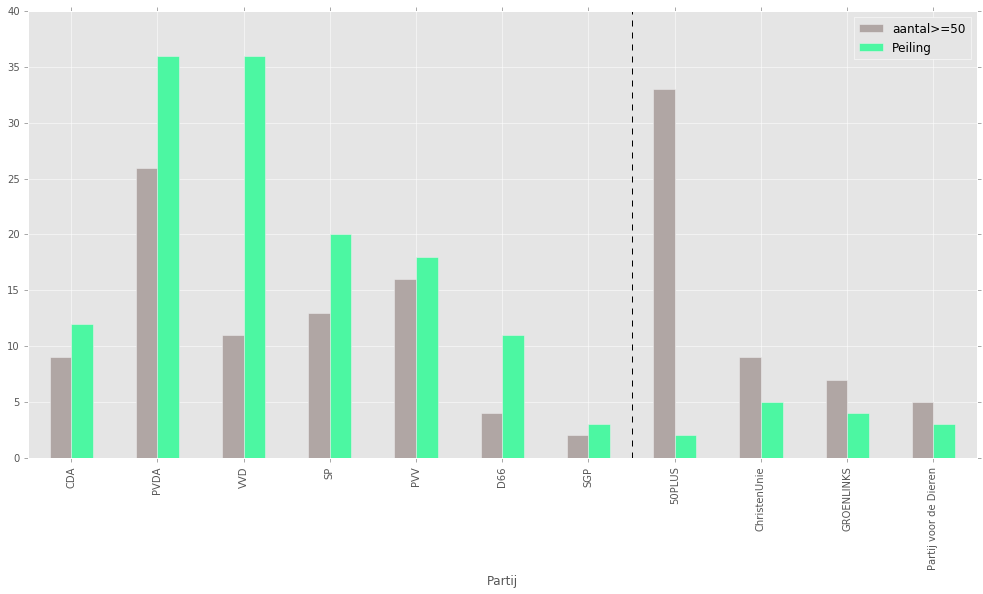
\includegraphics[width=0.98\linewidth]	{Aantal_ouderen_aantal_zetels.png}

			\caption{Het aantal ouderen op de kandidatenlijst(grijs) en het aantal zetels volgens de peilingen(groen) per partij.}

\label{fig:zetelsO}
\end{figure}

\paragraph{Maximaal aantal ouderen per partij(top \textit{N}) dat in de Tweede Kamer gekozen kan worden.}
In Tabel \ref{table:tab3O} hieronder is, in het verlengde van Figuur \ref{fig:zetelsO} hierboven, te zien hoeveel oudere kandidaten er per partij maximaal in de Tweede Kamer gekozen hadden kunnen worden. In de Tabel is dus per partij het aantal (\textit{N}) oudere kandidaten te zien waarover de stemmen van de oudere kiezers op de partij verdeeld zullen worden.  
\\
\indent Vanwege het feit dat het CDA, D66, de PVDA, de PVV, de SGP, de SP en de VVD volgens de peiling meer zetels gaan ontvangen dan zij ouderen op de kandidatenlijst hebben staan, komt het totaal aantal oudere kandidaten dat volgens de peiling in de Tweede Kamer gestemd kan worden op 95.




\begin{table}[h]
\centering
	\begin{footnotesize}
		\begin{tabular}{lrr}
\toprule
{} &  Top \textit{N} Oudere Kandidaten &  Overgebleven Kandidaten \\
Partij                &                          &                          \\
\midrule
50PLUS                &                        2 &                        0 \\
CDA                   &                        9 &                        3 \\
ChristenUnie          &                        5 &                        0 \\
D66                   &                        4 &                        7 \\
GROENLINKS            &                        4 &                        0 \\
Partij v d Dieren &                        3 &                        0 \\
PVDA                  &                       26 &                       10 \\
PVV                   &                       16 &                        2 \\
SGP                   &                        2 &                        1 \\
SP                    &                       13 &                        7 \\
VVD                   &                       11 &                       25 \\
\midrule
Toaal				  & 						95&                        55\\
\bottomrule
\end{tabular}

	\end{footnotesize}
			\caption{Per partij de top \textit{N} oudere kandidaten en de overgebleven kandidaten met een leeftijd van onder de 50 jaar a.d.h.v. de peiling.}
\label{table:tab3O} 
\end{table}



\paragraph{Het toewijzen van de stemmen aan de oudere kandidaten op basis van de peiling en de einduitslag.}
Op dezelfde wijze als bij de andere strategie\"{e}n wijzen we de hier de oudere stemmen toe a.d.h.v. de peiling en a.d.h.v. de einduitslag (voor gedetailleerde uitleg zie \hyperref[S1V]{Strategie 1} in \hyperref[vrouwen]{Bevolkingsgroep: Vrouwen}). In Figuur \ref{fig:stemmenS1O} hieronder is zowel de toewijzing op basis van de peiling alsmede de toewijzing op basis van de einduitslag te zien.


\begin{figure}[H]

	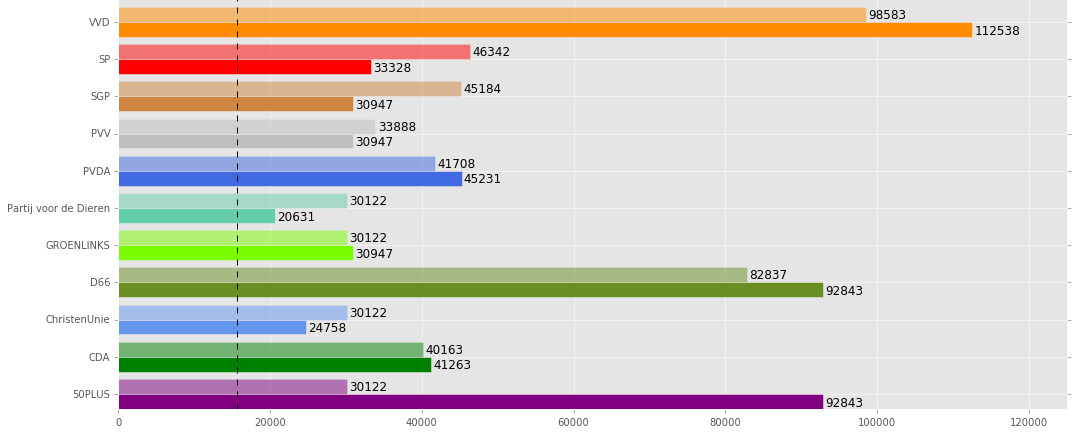
\includegraphics[width=\linewidth]	{stemmen_op_ouderen_topN_peiling.png}

			\caption{Grafiek met per partij de verdeling van de stemmen van oudere kiezers op alle oudere kandidaten van de partij a.d.h.v. de peiling (licht gekleurd) en a.d.h.v. de einduitslag (donker gekleurd). De stippellijn is de daadwerkelijk voorkeursdrempel(15.708 stemmen).}

\label{fig:stemmenS1O}
\end{figure}


Zoals te zien in Figuur \ref{fig:stemmenS1O} hierboven, zijn zowel volgens de peiling (voorspelling) alsmede volgens de einduitslag alle top \textit{N} oudere kandidaten van de partijen boven de daadwerkelijke voorkeursdrempel uitgekomen. Ofschoon de precieze aantallen niet exact hetzelfde zijn, is met strategie 2 de voorspelling zoals berekend a.d.h.v. de peiling correct in het voorspellen welke partijen met alle oudere kandidaten boven de voorkeursdrempel uitkomen en welke partijen dit niet het geval is.

\paragraph{Aantal ouderen na strategie 1.}
Na het uitvoeren van de strategie 1 en het opstellen van de Tweede Kamer zoals eerder in dit hoofdstuk beschreven, levert strategie 1 een Tweede Kamer op waarin  89 ouderen en 61 personen van onder de 50 jaar plaatsnemen. Daarmee zijn ouderen (met 59\%) ruim in betere mate vertegenwoordigd dan personen van onder de 50 jaar (met 41\%). In de cirkeldiagram in Figuur \ref{fig:pcS1O} hieronder is de verdeling goed te zien. 

\begin{figure}[H]
\centering
	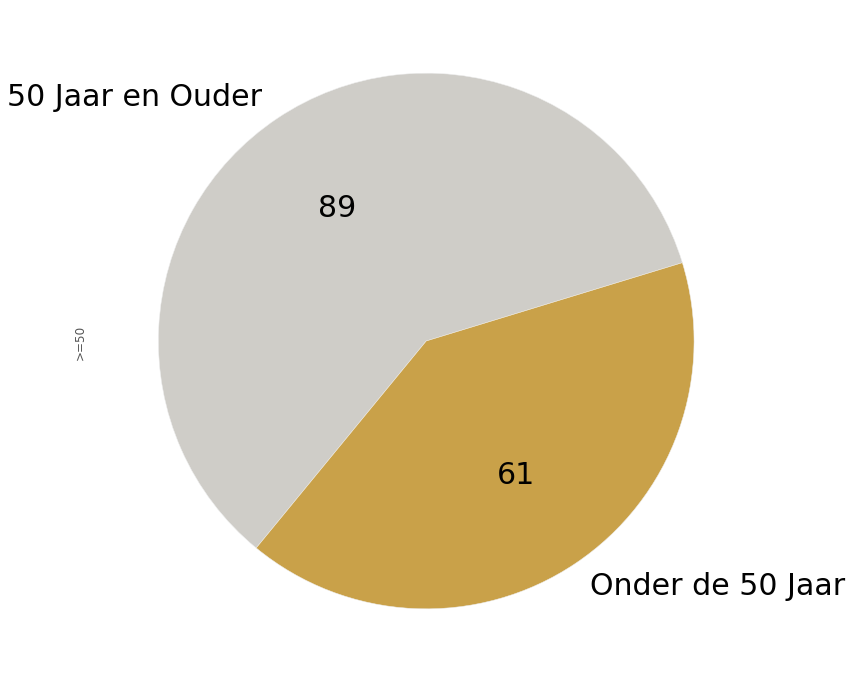
\includegraphics[width=0.42\linewidth]{pie_chart_topN_ouderen.png}

			Figuur ??: Na uitvoering van de strategie nemen er 89 ouderen(59\%) en 61 personen onder de 50 (41\%) plaats in de Tweede Kamer. 

\label{fig:pcS1O}
\end{figure}

\paragraph{Minder vrouwen dan 95 ouderen in de Tweede Kamer na uitvoering van strategie 1.}
De reden dat er niet 95 ouderen maar 'slechts' 89 ouderen in de Tweede Kamer plaatsnemen na uitvoering van strategie 1 ligt ten grondslag aan een aantal factoren. Bij GROENLINLS had de lijstrekker, in de persoon van Jolande 
Sap, meer stemmen dan de oudere kandidaten. Hierdoor viel bij GROENLINKS één oudere kandidaat af. De Partij voor de Dieren had de lijsttrekker, in de persoon van Marianne Thieme, ook meer stemmen dan de oudere kandidaten. Tevens ontving de Partij voor de Dieren één zetel minder bij de einduitslag dan dat de peiling aangaf. Hierdoor vielen er bij de Partij voor de Dieren twee oudere kandidaten af. Bij de PVV hadden zowel de lijsttrekker (Geert Wilders) als de nummer twee op de lijst (Fleur Agema) meer stemmen dan de oudere kandidaten. Tevens ontving de PVV drie zetels minder bij de einduitslag dan dat de peiling aangaf. Hierdoor vielen er bij de PVV drie oudere kandidaten af. Het aantal ouderen in de Tweede Kamer na uitvoering van strategie 1 komt daarom uit op ($95-6$ = ) 89. 




\subsubsection{Strategie 2: Oudere kiezers stemmen op een willekeurige oudere kandidaat.}




\paragraph{Het toewijzen van de stemmen aan de oudere kandidaten op basis van de peiling en de einduitslag.}
Op dezelfde wijze als bij de andere strategie\"{e}n wijzen we de hier de oudere stemmen toe a.d.h.v. de peiling en a.d.h.v. de einduitslag (voor gedetailleerde uitleg zie \hyperref[S1V]{Strategie 1} in \hyperref[vrouwen]{Bevolkingsgroep: Vrouwen}). In Figuur \ref{fig:stemmenS2O} hieronder is zowel de toewijzing op basis van de peiling alsmede de toewijzing op basis van de einduitslag te zien.


\begin{figure}[H]

	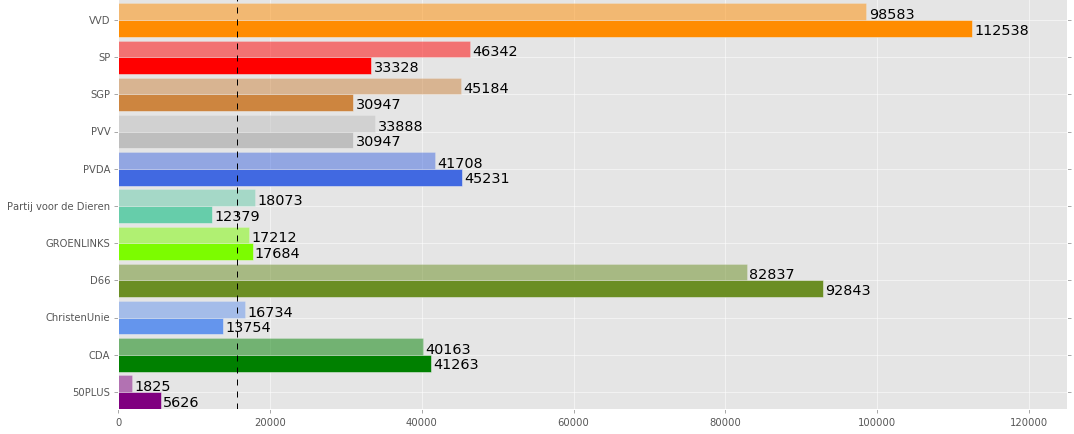
\includegraphics[width=\linewidth]	{stemmen_op_ouderen_willekeurig_samen.png}

			\caption{Grafiek met per partij de verdeling van de stemmen van oudere kiezers op alle oudere kandidaten van de partij a.d.h.v. de peiling (licht gekleurd) en a.d.h.v. de einduitslag (donker gekleurd). De stippellijn is de daadwerkelijk voorkeursdrempel(15.708 stemmen).}

\label{fig:stemmenS2O}
\end{figure}

Zoals te zien in Figuur\ref{fig:stemmenS2O} hierboven, zijn zowel volgens de peiling (voorspelling) alsmede volgens de einduitslag niet alle oudere kandidaten van de partijen boven de daadwerkelijke voorkeursdrempel uitgekomen. Ofschoon de precieze aantallen niet exact hetzelfde zijn, is met strategie 2 de voorspelling zoals berekend a.d.h.v. de peiling grotendeels correct in het voorspellen welke partijen met alle oudere kandidaten boven de voorkeursdrempel uitkomen en welke partijen dit niet het geval is. Enkel bij de Partij voor de Dieren en bij de ChristenUnie is er voorspeld dat de oudere kandidaten boven de voorkeursdrempel uit zouden komen terwijl niet bij de einduitslag niet zo blijkt te zijn.

\paragraph{Aantal ouderen na strategie 2.}
Na het uitvoeren van de strategie 2 en het opstellen van de Tweede Kamer zoals eerder in dit hoofdstuk beschreven, levert strategie 2 een Tweede Kamer op waarin 84 ouderen  en 66 personen onder de 50 jaar  plaatsnemen. Daarmee zijn ouderen (met 56\%) ruim in betere mate vertegenwoordigd dan personen van onder de 50 jaar (met 44\%). In de cirkeldiagram in Figuur \ref{fig:pcS2O} hieronder is de verdeling goed te zien. 


\begin{figure}[H]
\centering
	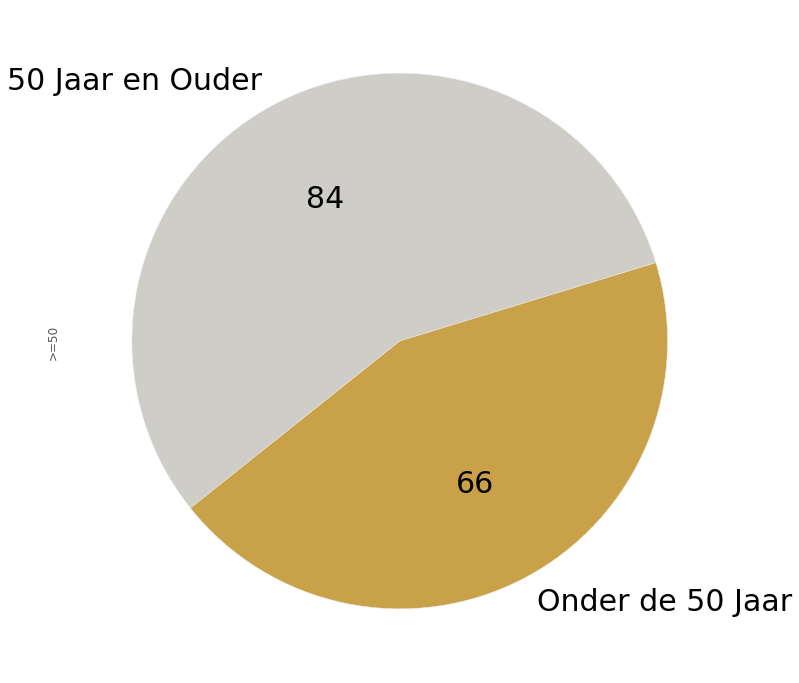
\includegraphics[width=0.42\linewidth]{pie_chart_willekeurig_ouderen.png}

			\caption{Na uitvoering van de strategie nemen er 84 ouderen(56\%) en 66 personen onder de 50(44\%) plaats in de Tweede Kamer.}

\label{fig:pcS2O}
\end{figure}





\paragraph{Één oudere minder in de Tweede Kamer ten opzicht van strategie 1.}
De reden dat er niet 89 maar 84 ouderen in de Tweede Kamer plaatsnemen na uitvoering van strategie 2 ligt ten grondslag aan een aantal factoren. Bij de Partij voor de Dieren en bij de ChristenUnie kregen de oudere kandidaten niet genoeg stemmen om boven de voorkeursdrempel van 15.708 stemmen uit te komen. Hierdoor viel er bij deze partijen in totaal vijf oudere kandidaten af. Hoewel ook bij 50PLUS de oudere kandidaten ook te weinig stemmen kregen om boven de voorkeursdrempel uit te komen, had 50PLUS enkel ouderen op de kandidatenlijst staan. Hierdoor vallen er bij 50PLUS geen oudere kandidaten af. 




%\titlespacing*{\subsubsection}{0pt}{30pt}{10pt}
\subsubsection{Strategie 3.1: Oudere kiezers stemmen willekeurige op één van de eerste 15 oudere kandidaten van een partij.}

\paragraph{Partijen met minstens 15 oudere kandidaten en partijen met minder dan 15 oudere kandidaten.}
In de grafiek in Figuur \ref{fig:15O} hieronder zien we dat bij 50PLUS, de PVDA en de PVV de stemmen van oudere kiezers over de top 15 oudere kandidaten verdeeld kunnen worden. Bij de overige partijen moeten de stemmen van oudere kiezers die de partij volgens de peiling zou gaan ontvangen verdeeld worden over alle oudere kandidaten die deze partijen op hun kandidatenlijsten hadden staan.




\begin{figure}[H]

	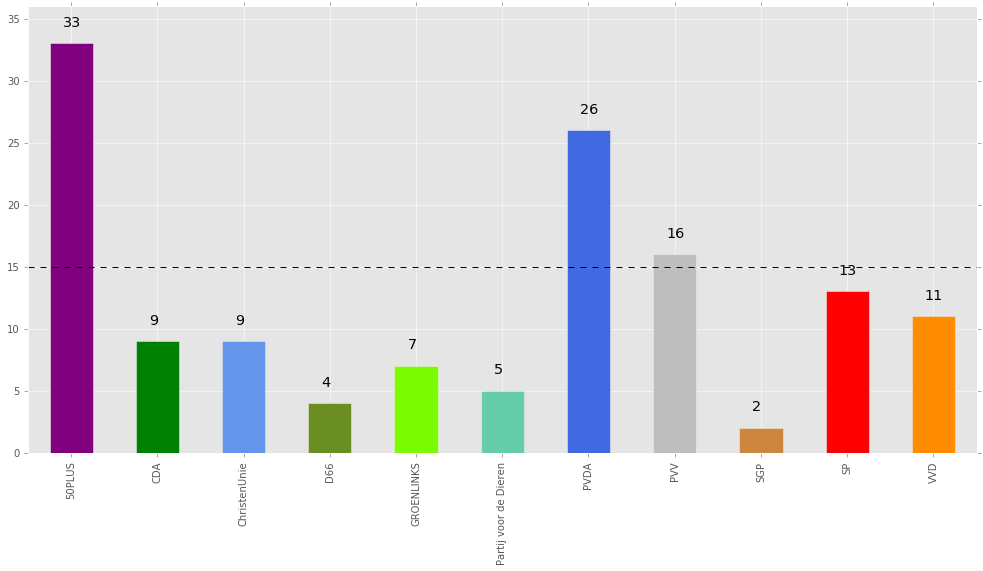
\includegraphics[width=\linewidth]	{top15_of_topN_kandidaten_ouderen.png}

			\caption{De grafiek toont bij welke partijen de oudere kiezers op de top 15 oudere kandidaten van de partij kunnen gaan stemmen (\textit{N=15}) en van welke partijen de oudere kiezers op alle oudere kandidaten van de partij kunnen gaan stemmen (\textit{N=totaal aantal oudere kandidaten}).} 


\label{fig:15O}
\end{figure}



\paragraph{Het toewijzen van de stemmen aan de oudere kandidaten op basis van de peiling en de einduitslag.}
Op dezelfde wijze als bij de andere strategie\"{e}n wijzen we de hier de oudere stemmen toe a.d.h.v. de peiling en a.d.h.v. de einduitslag (voor gedetailleerde uitleg zie \hyperref[S1V]{Strategie 1} in \hyperref[vrouwen]{Bevolkingsgroep: Vrouwen}). In Figuur \ref{fig:stemmenS31O} hieronder is zowel de toewijzing op basis van de peiling alsmede de toewijzing op basis van de einduitslag te zien.

\begin{figure}[H]

	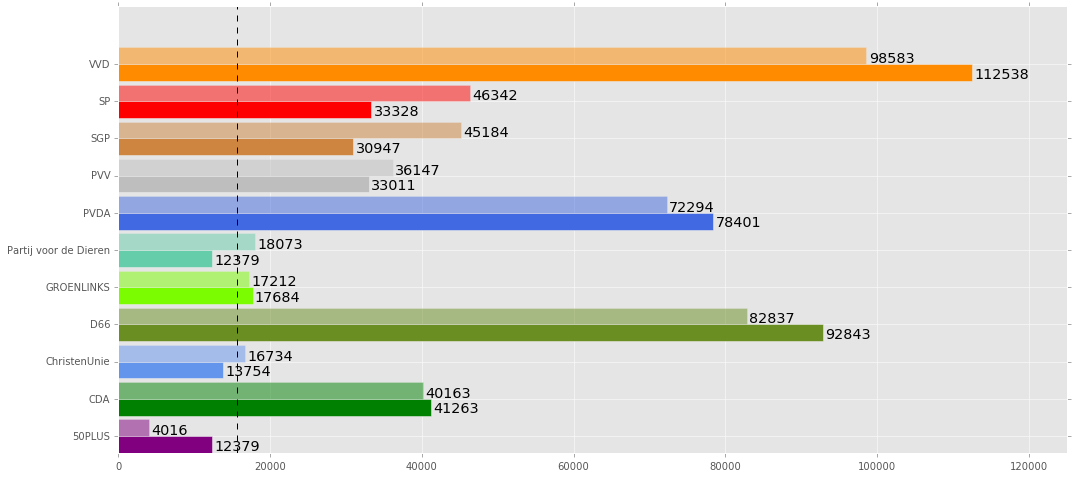
\includegraphics[width=\linewidth]	{stemmen_op_ouderen_top15_of_topN_samen.png}

			\caption{Grafiek met per partij de verdeling van de stemmen van vrouwelijk kiezers op alle vrouwelijke kandidaten van de partij a.d.h.v. de peiling (licht gekleurd) en a.d.h.v. de einduitslag (donker gekleurd). De stippellijn is de daadwerkelijk voorkeursdrempel(15.708 stemmen).}

\label{fig:stemmenS31O}
\end{figure}

Zoals te zien in Figuur \ref{fig:stemmenS31O} hierboven, zijn zowel volgens de peiling (voorspelling) alsmede volgens de einduitslag niet alle oudere kandidaten van de partijen boven de daadwerkelijke voorkeursdrempel uitgekomen. Ofschoon de precieze aantallen niet exact hetzelfde zijn, is met strategie 3.1 de voorspelling zoals berekend a.d.h.v. de peiling grotendeels correct in het voorspellen welke partijen welke partijen met de top \textit{N} (\textit{N=15} of \textit{N=totaal aantal oudere kandidaten}) oudere kandidaten boven de voorkeursdrempel uitkomen en welke partijen dit niet het geval is. Enkel bij de Partij voor de Dieren en bij de ChristenUnie is er voorspeld dat de top \textit{N} oudere kandidaten boven de voorkeursdrempel uit zouden komen terwijl niet bij de einduitslag niet zo blijkt te zijn.

\paragraph{Aantal ouderen na strategie 3.1.}
Na het uitvoeren van de strategie 3.1 en het opstellen van de Tweede Kamer zoals eerder in dit hoofdstuk beschreven, levert strategie 3.1 uiteindelijk een Tweede Kamer op waarin 73 ouderen en 77 personen onder 50 jaar plaatsnemen. Daarmee zijn ouderen(met 49\%) net aan in mindere mate vertegenwoordigd dan personen van onder de 50 jaar(met 51\%). In de cirkeldiagram in Figuur \ref{fig:pcS31O} hieronder is de verdeling goed te zien. In de volgende paragraaf wordt uitgelegd waarom er niet 84 (zoals in de vorige strategie) maar slechts 73 ouderen in de Tweede Kamer Plaatsnemen na uitvoering van strategie 3.1 ten opzichte van strategie 2.

\begin{figure}[H]
\centering
	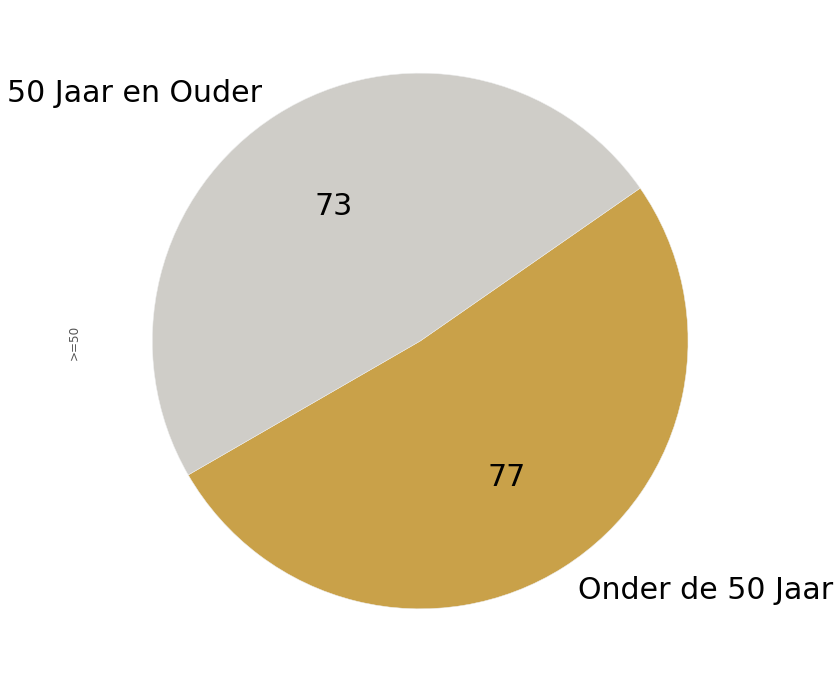
\includegraphics[width=0.42\linewidth]{pie_chart_top15_of_topN_ouderen.png}

			\caption{Na uitvoering van de strategie nemen er 73 ouderen (49\%) en 77 personen onder de 50 jaar (51\%) plaats in de Tweede Kamer.}

\label{fig:pcS31O}
\end{figure}

\paragraph{Minder vrouwen in de Tweede Kamer d.m.v. uitvoering van strategie 3.1 dan d.m.v. uitvoering van strategie 2.}
De reden dat er, na uitvoering van strategie 3.1, 73 ouderen in de Tweede Kamer plaatsnemen en dat er daarmee elf ouderen minder plaatsnemen in de Tweede Kamer dan bij strategie 2 het geval zou zijn ligt ten grondslag aan het feit dat er bij de PVDA elf oudere kandidaten afvallen ten opzichte van strategie 2. Dit komt omdat de stemmen niet verdeeld worden over alle 26 oudere kandidaten van de PVDA maar over de top 15 oudere kandidaten van de PVDA. De overige elf oudere kandidaten van de PVDA staan niet hoog genoeg op de kandidatenlijst om een zetel te ontvangen. Daarmee komt het totale aantal ouderen in de Tweede Kamer uit op ($84-11$ = ) 73.






\subsubsection{Strategie 3.2: Oudere kiezers stemmen willekeurige op één van de eerste \textit{N} oudere kandidaten van een partij.}


\paragraph{Voor elke partij de eigen \textit{N} bepalen.}
Hieronder is in de grafiek in Figuur \ref{fig:XO} per partij te zien op welke waarde het \textit{N} oudere kandidaten wordt bepaald. Het CDA, de ChristenUnie, GROENLINKS en de Partij voor de Dieren hebben allemaal minder dan tien oudere kandidaten op de kandidatenlijst staan en daardoor geldt voor deze partijen \textit{N=5}. Ook de SGP en D66 hebben minder dan tien oudere kandidaten op de kandidatenlijst. Deze partijen hebben echter zelfs minder dan vijf oudere kandidaten op de kandidatenlijst staan. Hierdoor geld voor deze partijen een \textit{N=totaal aantal oudere kandidaten}. Voor de SGP geldt \textit{N=2} en voor D66 geldt \textit{N=4}. De SP en de VVD hebben tien of meer vrouwelijke kandidaten op de kandidatenlijsten maar minder dan vijftien. Hierdoor geldt voor deze partijen \textit{N=10}. De PVDA en de PVV hebben vijftien of meer oudere kandidaten op de kandidatenlijsten maar minder dan dertig. Hierdoor geldt voor deze partijen \textit{N=30}. Enkel de 50PLUS heeft meer dan dertig oudere kandidaten op de kandidatenlijst staan en daardoor geldt voor 50PLUS \textit{N=30}. 

\begin{figure}[H]

	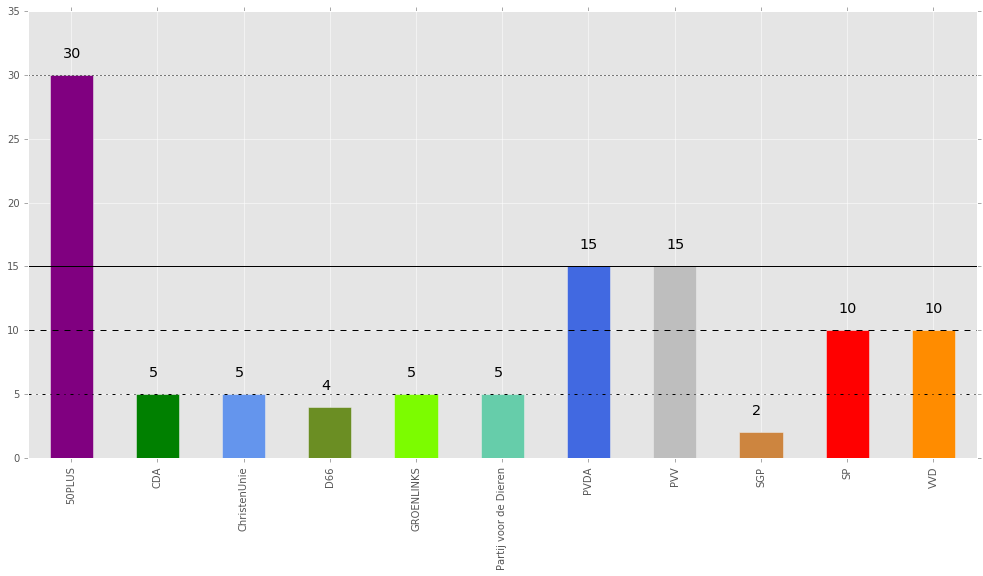
\includegraphics[width=\linewidth]{eigenX_partijen_ouderen.png}
		\caption{Elke partij krijgt een eigen \textit{N}. De lijnen geven een mogelijke \textit{N} aan.}

\label{fig:XO}
\end{figure}





\paragraph{Het toewijzen van de stemmen aan de oudere kandidaten op basis van de peiling en de einduitslag.}
Op dezelfde wijze als bij de andere strategie\"{e}n wijzen we de hier de oudere stemmen toe a.d.h.v. de peiling en a.d.h.v. de einduitslag (voor gedetailleerde uitleg zie \hyperref[S1V]{Strategie 1} in \hyperref[vrouwen]{Bevolkingsgroep: Vrouwen}). In Figuur \ref{fig:stemmenS32O} hieronder is zowel de toewijzing op basis van de peiling alsmede de toewijzing op basis van de einduitslag te zien.


\begin{figure}[H]

	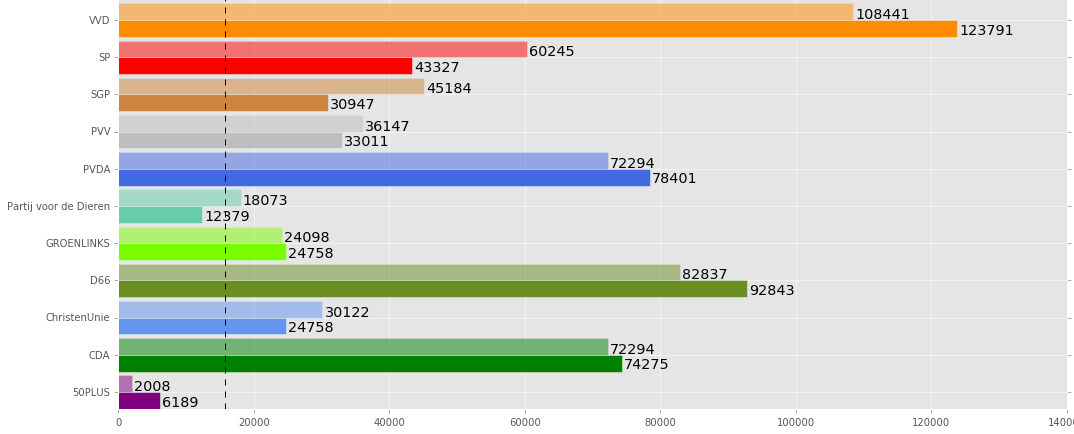
\includegraphics[width=\linewidth]{stemmen_op_ouderen_eigenX_samen.png}

			\caption{Grafiek met per partij de verdeling van de stemmen van vrouwelijk kiezers op alle vrouwelijke kandidaten van de partij a.d.h.v. de peiling (licht gekleurd) en a.d.h.v. de einduitslag (donker gekleurd). De stippellijn is de daadwerkelijk voorkeursdrempel(15.708 stemmen).}

\label{fig:stemmenS32O}
\end{figure}

Zoals te zien in Figuur \ref{fig:stemmenS32O} hierboven, zijn zowel volgens de peiling (voorspelling) alsmede volgens de einduitslag niet alle oudere kandidaten van de partijen boven de daadwerkelijke voorkeursdrempel uitgekomen. Ofschoon de precieze aantallen niet exact hetzelfde zijn, is met strategie 3.2 de voorspelling zoals berekend a.d.h.v. de peiling grotendeels correct in het voorspellen welke partijen welke partijen met de top \textit{N} (\textit{N=5}, \textit{N=10}, \textit{N=15}, \textit{N=30} of \textit{N=totaal aantal oudere kandidaten}) oudere kandidaten boven de voorkeursdrempel uitkomen en welke partijen dit niet het geval is. Enkel is ook bij strategie 3.2 voor de Partij voor de Dieren voorspeld dat de top \textit{N} oudere kandidaten (voor de Partij voor de Dieren geldt \textit{N=5}) boven de voorkeursdrempel uit zouden komen terwijl niet bij de einduitslag niet zo blijkt te zijn.  Dit ligt ten grondslag aan het feit dat de Partij voor de Dieren een kleiner aantal stemmen kreeg dan de peiling had voorspeld. 


\paragraph{Aantal ouderen na strategie 3.2.}
Na het uitvoeren van de strategie 3.2 en het opstellen van de Tweede Kamer zoals eerder in dit hoofdstuk beschreven, levert strategie 3.2 een Tweede Kamer op waarin 69 ouderen en 81 personen onder de 50 jaar plaatsnemen. Daarmee zijn ouderen (met 46\%) in mindere mate vertegenwoordigd dan personen onder de 50 jaar (met 54\%). In de cirkeldiagram in Figuur \ref{fig:pcS32O} hieronder is de verdeling goed te zien. In de volgende paragraaf wordt uitgelegd waarom er acht ouderen minder in de Tweede Kamer plaatsnemen na uitvoering van strategie 3.2 ten opzicht van strategie 3.1.

\begin{figure}[H]
\centering
	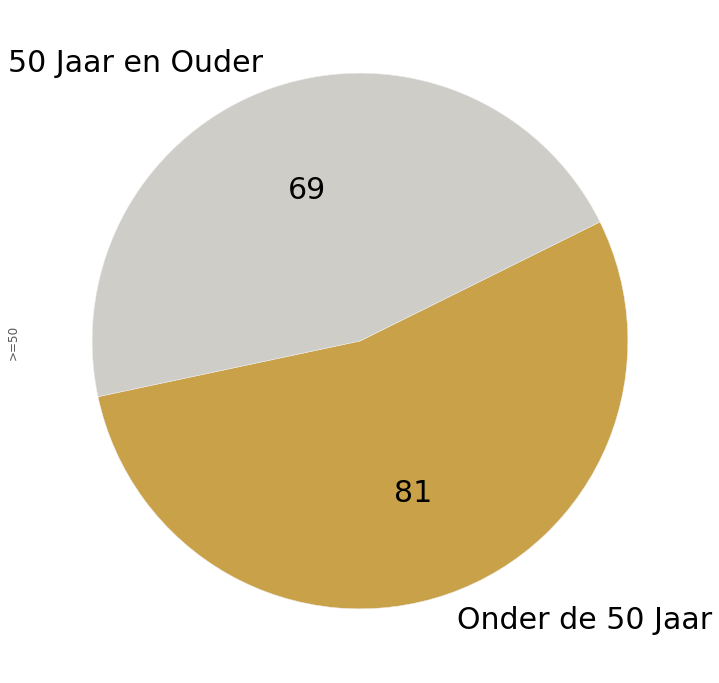
\includegraphics[width=0.40\linewidth]{pie_chart_eigenX_ouderen.png}

\caption{Na uitvoering van de strategie nemen er 69 ouderen(58.7\%) en 81 personen onder de 50(41.3\%) plaats in de Tweede Kamer.} 

\label{fig:pcS32O}
\end{figure}

\paragraph{Meer vrouwen in de Tweede Kamer d.m.v. uitvoering van strategie 3.2 dan d.m.v. uitvoering van strategie 3.1.}
De reden dat er, na uitvoering van strategie 3.2, 69 ouderen in de Tweede Kamer plaatsnemen en dat er daarmee vier ouderen minder zijn ten opzichte van strategie 3.1 ligt ten grondslag aan het feit dat bij het CDA vier oudere kandidaten afvallen. Het CDA had negen oudere kandidaten op de kandidatenlijst. Door uitvoering van strategie 3.2 worden de oudere stemmen op het CDA echter verdeeld over de top vijf oudere kandidaten van het CDA. Op dezelfde manier vielen er bij de SP drie oudere kandidaten af (dertien oudere kandidaten op de kandidatenlijst, tien oudere kandidaten waarover de oudere stemmen verdeeld zijn) en bij de VVD viel één oudere kandidaat af (elf oudere kandidaten op de kandidatenlijst, tien oudere kandidaten waarover de oudere stemmen verdeeld zijn). De oudere top 5 oudere kandidaten van de ChristenUnie kwamen met strategie 3.2 echter wel boven de kiesdrempel. Hierdoor komen er vier ouderen voor de ChristenUnie in de Tweede Kamer bij. Daarmee komt het totale aantal ouderen in de Tweede Kamer uit op ($73-4$ = )69.








\subsubsection{Strategie 4: Ouderen kiezers stemmen op de top \textit{N+extra percentage} oudere kandidaten van een partij.}

\paragraph{Speling in top \textit{N}.}
Zoals te zien in Figuur \ref{fig:zetelsO}, zijn er meerdere partijen die een hoger aantal oudere kandidaten op de kandidatenlijst hebben staan dan dat verwacht werd dat zij, volgens de peiling, aan zetels zouden gaan ontvangen. Vanwege het feit dat de zetelverdeling volgens de peiling niet 100\% correspondeerde met de zetelverdeling volgens de einduitslag, is het ook voor de bevolkingsgroep ouderen interessant om te kijken wat er gebeurt wanneer de top \textit{N} wordt uitgebreid met een \textit{extra percentage} bovenop de eerder al per partij bepaalde top \textit{N} uit strategie 1.



\paragraph{Maximaal aantal ouderen per partij(top \textit{N+extra percentage}) dat in de Tweede Kamer gekozen kan worden.} 
Bij strategie 4 wordt de top \textit{N} voor elke partij uitgebreid met een \textit{extra percentage} van \textit{N} in stappen van 10\% extra (dus eerst 110\%, dan 120\% etc.). Zodoende worden de oudere stemmen die een partij ontvangt telkens over de top \textit{N+extra percentage} oudere kandidaten van de partij verdeeld. Daarbij kan de top \textit{N+extra percentage} van een partij nooit meer worden dat het totaal aantal oudere kandidaten dat de partij op de kandidatenlijst heeft staan. In Figuur \ref{fig:NexpO} hieronder is er per partij te zien wat er met de top \textit{N} gebeurt wanneer het \textit{extra percentage} hieraan wordt toegevoegd.  


\begin{figure}[H]

	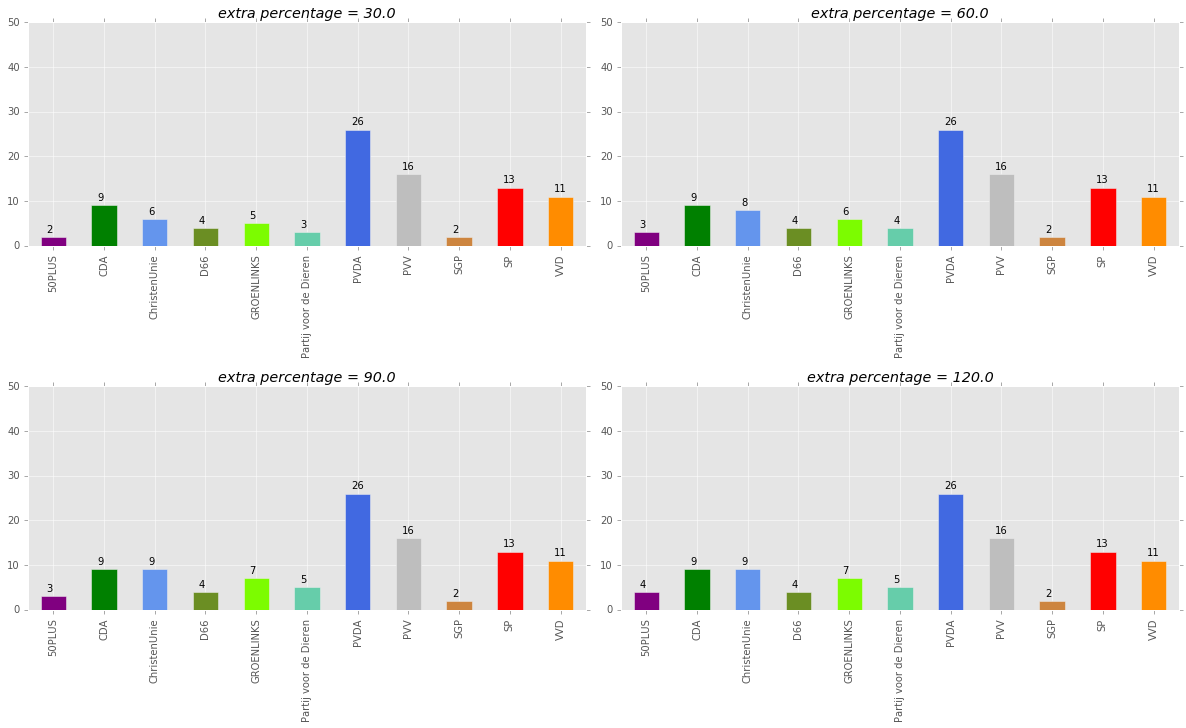
\includegraphics[width=\linewidth]{topN_vermenigvuldiging_ouderen.png}

			\caption{De top \textit{N+extra percentage} waarin \textit{extra percentage} respectievelijk 30\%, 60\%, 90\% en 120\% extra te verwachten zetels (voor vrouwelijke kandidaten)  zijn.}

\label{fig:NexpO}
\end{figure}



\paragraph{Het toewijzen van de stemmen aan de oudere kandidaten op basis van de peiling en de einduitslag.}
Op dezelfde wijze als bij de andere strategie\"{e}n wijzen we de hier de oudere stemmen toe a.d.h.v. de peiling en a.d.h.v. de einduistlag (voor gedetailleerde uitleg zie \hyperref[S1V]{Strategie 1} in \hyperref[vrouwen]{Bevolkingsgroep: Vrouwen}). In de grafieken in Figuur \ref{fig:stemmenS4O} hieronder is zowel de toewijzing van vrouwelijke stemmen op vrouwelijke kandidaten op basis van de peiling alsmede op basis van de einduitslag voor alle partijen te zien. De toewijzingen worden getoond aan de hand van respectievelijk 30\%, 60\%, 90\% en 120\% (\textit{extra percentage}) extra zetels (voor vrouwelijke kandidaten) waarover de stemmen verdeeld worden.

  
\begin{figure}[H]

	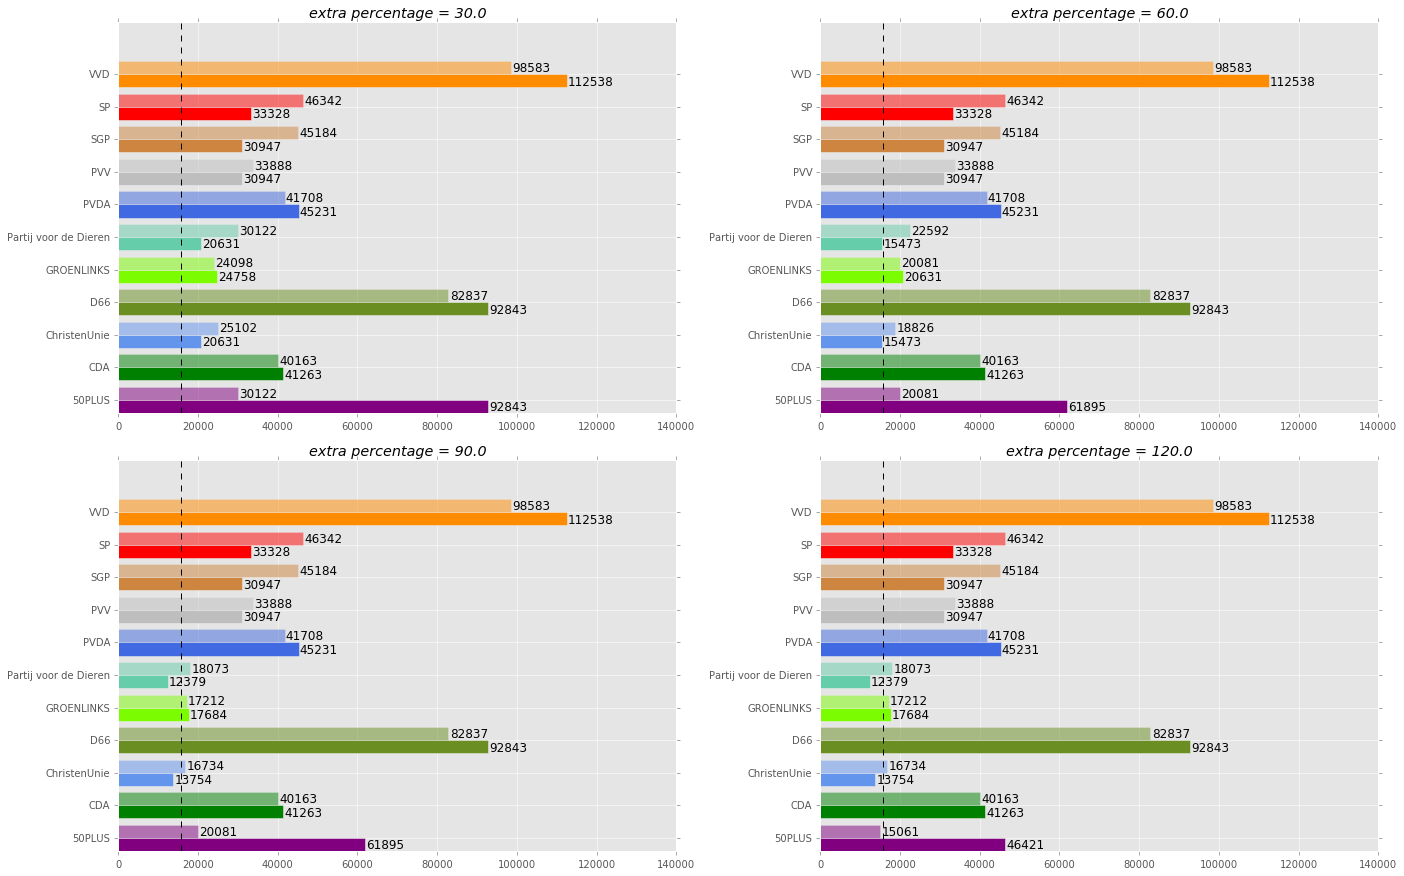
\includegraphics[width=\linewidth]	{stemmen_op_ouderen_topNextrapercentage_samen.png}

			\caption{Grafieken in stappen van 30\%, met per partij de verdeling van de stemmen van vrouwelijke kiezers op de top \textit{N+extra percentage} vrouwelijke kandidaten van de partij a.d.h.v. de peiling (licht gekleurd) en a.d.h.v. de einduitslag (donker gekleurd). De stippellijn is de daadwerkelijk voorkeursdrempel(15.708 stemmen).} 

\label{fig:stemmenS4O}
\end{figure}

In Figuur \ref{fig:stemmenS4O} hierboven, is te zien dat zowel volgens de peiling (voorspelling) alsmede volgens de einduitslag niet alle top \textit{N+extra percentage} oudere kandidaten van de partijen boven de daadwerkelijke voorkeursdrempel uitgekomen wanneer het \textit{extra percentage} aan zetels (voor oudere kandidaten) wordt verhoogd. Echter gebeurt dit pas tussen de 30\%  en 60\% extra zetels (voor oudere kandidaten) waarover de stemmen verdeeld worden. Ofschoon de precieze aantallen niet exact hetzelfde zijn, is met strategie 4 de voorspelling zoals berekend a.d.h.v. de peiling grotendeels correct in het voorspellen welke partijen met de top \textit{N+extra percentage} vrouwelijke kandidaten boven de voorkeursdrempel uitkomen en van welke partijen dit niet het geval is.



\paragraph{Aantal ouderen na strategie 4.}
Na het uitvoeren van strategie 4 en het opstellen van de Tweede Kamer zoals eerder in dit hoofdstuk beschreven, levert strategie 4 bij geen enkel \textit{extra percentage} bovenop de originele \textit{N} uit strategie 1 een hoger aantal ouderen op in de Tweede Kamer. In de grafiek hieronder in Figuur \ref{fig:bcS4O}  is te zien hoeveel vrouwen er in de Tweede Kamer een zetels bedeeld krijgen wanneer er een bepaald \textit{extra percentage} wordt toegevoegd aan de originele \textit{N} uit strategie 1.



\begin{figure}[H]

	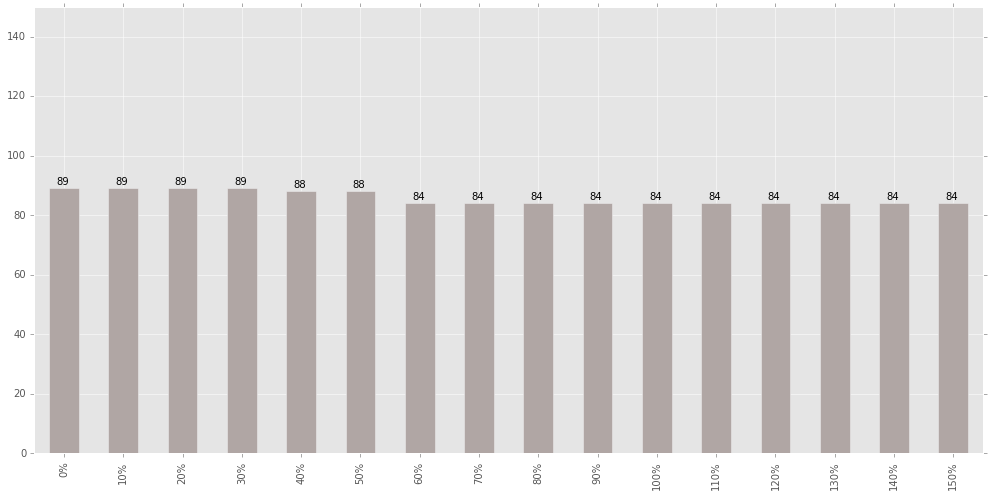
\includegraphics[width=\linewidth]	{topNextrapercentage_aantal_ouderen_overzicht.png}

			\caption{Grafiek met per het aantal ouderen in de Tweede Kamer na uitvoering(en) van strategie 4 in stappen van 10\% aan \textit{extra percentage} (van \textit{N}) bovenop de \textit{N} uit strategie 1. }

\label{fig:bcS4O}
\end{figure}

\paragraph{Niet meer maar minder ouderen na uitvoering van strategie 4.}
Zoals hierboven in Figuur \ref{fig:bcS4O} te zien, komen er na uitvoering van strategie 4 en het toenemen van het \textit{extra percentage} op geen enkel moment meer ouderen in de Tweede Kamer dan de 121 uit strategie 1 (0\% staat in de grafiek gelijk aan strategie 1.) 


\paragraph{Niet meer dan 89 ouderen in de Tweede Kamer.}
De reden dat er niet meer dan 89 ouderen in de Tweede Kamer plaatsnemen na uitvoering van strategie 4 ligt ten grondslag aan een aantal factoren. Willen er meer ouderen in de Tweede Kamer plaatsnemen dan na uitvoering van strategie 1 dan is het noodzakelijk dat de partijen ook meer zetels kregen bedeeld bij de einduitslag dan dat volgens te peiling was te verwachten. 
\\
\indent
Zo hadden de meeste partijen een kleiner aantal (of een gelijk aantal) ouderen op de kandidatenlijst staan als dat de peiling aangaf dat zij aan zetels zouden gaan ontvangen. Hierdoor werd de top \textit{N} van deze partijen niet uitgebreid wanneer het \textit{extra percentage} aan de \textit{N} werd toegevoegd. De Partij voor de Dieren, 50PLUS, de ChristenUnie en GROENLINKS kregen bij de einduitslag niet meer zetels dan volgens de peiling werd verwacht. Zodoende kan het aantal ouderen die in de Tweede Kamer plaatsnemen nooit op meer dan 89 uitkomen.


\subsection{Bevolkingsgroep: Provincialen.} \label{provincialen}
Betreffende de bevolkingsgroep provincialen in Nederland worden hieronder de resultaten van de verschillende strategie\"{e}n uiteengezet om zodoende te achterhalen met welke strategie in theorie de meeste provinciale kandidaten in de Tweede Kamer gekozen kunnen worden wanneer alle stemgerechtigde provincialen kiezers in Nederland zich committeren aan de strategie.\\
\indent Ten behoeve van de leesbaarheid worden er geen voorbeelden gegeven betreffende berekeningen. Alle voorbeelden zijn te vertalen vanuit de bij de bevolkingsgroep vrouwen toegepaste strategie\"{e}n (zie Sectie \ref{vrouwen}). 

\paragraph{Aannames en Regels.}
De aannames en regels zijn hetzelfde als bij de strategie\"{e}n voor de bevolkingsgroep vrouwen . Hierbij moet genoteerd worden dat vrouwen vervangen dient te worden voor provincialen en provinciale kandidaten vervangen dient te worden voor provinciale kandidaten (voor een gedetailleerde omschrijving van de aannames zie Sectie \hyperref[besS]{Beschrijving Strategie\"{e}n} en voor de regels van een strategie zie correspondeerde strategie in Sectie \ref{vrouwen})..

\paragraph{Het berekenen van het aantal te verwachten provinciale stemmen.}
\iffalse
Eerder in dit hoofdstuk wordt er in detail aan de hand van enkele voorbeelden uitgelegd hoe het aantal te verwachten vrouwelijke stemmen kan worden berekend (zie Sectie \hyperref[vrouwen]{Bevolkingsgroep: Vrouwen}). In deze sectie wordt de bevolkingsgroep provincialen in Nederland behandeld. De manier van berekenen is hetzelfde bij de deze bevolkingsgroep als bij de bevolkingsgroep vrouwen in Nederland. 
\fi
Op 1 september 2012 waren er 8.438.199 stemgerechtigde provincialen wonenden in Nederland \citep{Kiesraad_uitslag}. Vanwege het ontbreken van een peiling onder de provinciale kiezers nemen we aan dat de provinciale kiezers hetzelfde stemgedrag vertonen als de Nederlandse kiezers vertoonden volgens de landelijke peiling. We gaan derhalve uit van een opkomst van 73\% (zoals de landelijke peiling aangaf). Dat komt neer op een aantal van (73\%*8.438.199 = ) 6.159.885 stemmen. Op dezelfde wijze als bij de bevolkingsgroepen allochtonen en ouderen, is voor de bevolkingsgroep provincialen berekend hoeveel stemmen de partijen van provinciale kiezers konden gaan verwachten (zie Sectie \ref{allochtonen} voor uitleg). In Tabel \ref{table:tab1P} hieronder is per partij te zien hoeveel procent van de provinciale kiezers op een partij heeft gestemd en het aantal stemmen dat een partij van provincialen heeft ontvangen.

\begin{table}[h]
\centering
	\begin{footnotesize}
		\begin{tabular}{lrr}
\toprule
{} &  Provinciale Stempercentage &  Aantal Stemmen Van Provincialen \\
Partij                &                             &                                  \\
\midrule
50PLUS                &                        1,33 &                            82130 \\
CDA                   &                        8,00 &                           492790 \\
ChristenUnie          &                        3,33 &                           205326 \\
D66                   &                        7,33 &                           451717 \\
GROENLINKS            &                        2,67 &                           164257 \\
Partij voor de Dieren &                        2,00 &                           123197 \\
PVDA                  &                       24,00 &                          1478372 \\
PVV                   &                       12,00 &                           739186 \\
SGP                   &                        2,00 &                           123197 \\
SP                    &                       13,33 &                           821312 \\
VVD                   &                       24,00 &                          1478372 \\
\midrule
Totaal					&					100	&								6.159.855\\
\bottomrule
\end{tabular}

	\end{footnotesize}
			\caption{Totaal aantal stemmen dat een partij zou gaan ontvangen en het totaal aantal te verwachten provinciale stemmen volgens de peiling.}
\label{table:tab1P} 
\end{table}


\paragraph{Het berekenen van het daadwerkelijke aantal provinciale stemmen.}
\iffalse
Eerder in dit hoofdstuk wordt er in detail aan de hand van enkele voorbeelden uitgelegd hoe het daadwerkelijke aantal vrouwelijke stemmen kan worden berekend (zie Bevolkingsgroep: Vrouwen). Ook hier is de manier van berekenen van het daadwerkelijke aantal provinciale stemmen hetzelfde als bij de bevolkingsgroep vrouwen.
\fi
Vanwege het ontbreken van een peiling onder provincialen was er ook geen prognose over de verwachte opkomst. Daarom hebben we de landelijke opkomstprognose van 73\% genomen. Echter was er een landelijke opkomst van 74,6\% \citep{Kiesraad_uitslag}. Het aantal uitgebrachte provinciale stemmen kom hiermee op ($74,6\%*8.438.199$ = ) 6.294.896 stemmen. Hieronder in Tabel \ref{table:tab2P} is per partij te zien hoeveel procent van de provinciale kiezers op de partij heeft gestemd en het aantal stemmen dat een partij van provincialen heeft ontvangen. Op dezelfde wijze als het berekenen aantal te verwachten allochtone stemmen (zie \hyperref[S1A]{strategie 1} in Sectie \ref{allochtonen}), is ook het daadwerkelijk aantal provinciale stemmen per partij berekend. 
   
\begin{table}[h]
\centering
	\begin{footnotesize}
		\begin{tabular}{lrr}
\toprule
{} &  Provinciale Stempercentage &  Aantal Provinciale Stemmen \\
Partij                &                             &                             \\
\midrule
50PLUS                &                        1,33 &                       83930 \\
CDA                   &                        8,67 &                      545557 \\
ChristenUnie          &                        3,33 &                      209828 \\
D66                   &                        8,00 &                      503591 \\
GROENLINKS            &                        2,67 &                      167863 \\
Partij voor de Dieren &                        1,33 &                       83931 \\
PVDA                  &                       25,33 &                     1594705 \\
PVV                   &                       10,00 &                      629489 \\
SGP                   &                        2,00 &                      125897 \\
SP                    &                       10,00 &                      629489 \\
VVD                   &                       27,33 &                     1720602 \\
\midrule
Totaal			&								100	&						6294889		\\
\bottomrule
\end{tabular}

	\end{footnotesize}
			\caption{Totaal aantal stemmen dat een partij heeft ontvangen, het aandeel stemmen van provincialen in percentage en het totaal aantal provinciale stemmen volgens de einduitslag.}
\label{table:tab2P} 
\end{table}

\subsubsection{Strategie 1: Provinciale kiezers stemmen op top \textit{N} Provinciale kandidaten.}
\label{sssec:S1P}


 
\paragraph{Verdelingen zetels en aantal Provinciale kandidaten.}
In de grafiek hieronder in Figuur \ref{fig:zetelsP} is te zien dat voor alle partijen links van de stippellijn de top \textit{N} gelijk is aan het aantal provinciale dat de partij op de kandidatenlijst had staan. Bij de partijen rechts van de stippellijn is \textit{N} gelijk aan het aantal te verwachten zetels volgens de peiling. 

 
\begin{figure}[H]

	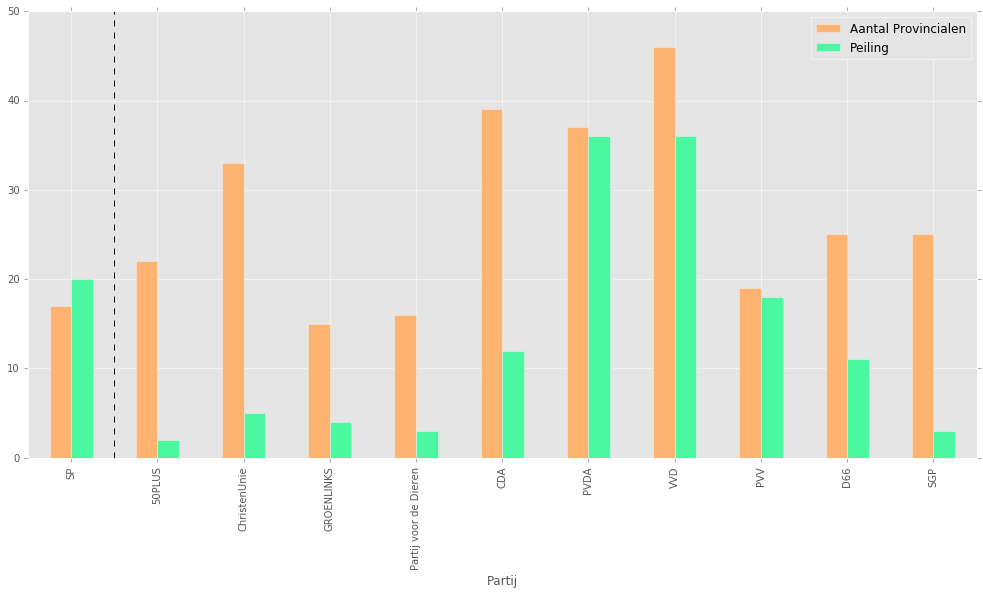
\includegraphics[width=\linewidth]	{Aantal_provincialen_aantal_zetels.png}

			\caption{Het aantal provinciale op de kandidatenlijst(grijs) en het aantal zetels volgens de peilingen(groen) per partij.}

\label{fig:zetelsP}
\end{figure}

\paragraph{Maximaal aantal provincialen per partij(top \textit{N}) dat in de Tweede Kamer gekozen kan worden.}
In Tabel \ref{table:tab3P} hieronder is, in het verlengde van Figuur \ref{fig:zetelsP}  hierboven, te zien hoeveel provinciale kandidaten er per partij maximaal in de Tweede Kamer gekozen hadden kunnen worden. In de Tabel is dus per partij het aantal (\textit{N}) provinciale kandidaten te zien waarover de stemmen van de provinciale kiezers op de partij verdeeld zullen worden.  
\\
\indent Vanwege het feit dat enkel de SP minder provinciale kandidaten op de kandidatenlijst heeft staan dan dat de partij volgens de peiling zou gaan ontvangen, komt het totaal aantal provinciale kandidaten dat volgens de peiling in de Tweede Kamer gekozen kan worden op 147.




\begin{table}[h]
\centering
	\begin{footnotesize}
		\begin{tabular}{lrr}
\toprule
{} &  Top N Provinciale Kandidaten &  Kandidaten Uit De Randstad \\
Partij                &                               &                             \\
\midrule
50PLUS                &                             2 &                         0 \\
CDA                   &                            12 &                         0 \\
ChristenUnie          &                             5 &                         0 \\
D66                   &                            11 &                         0 \\
GROENLINKS            &                             4 &                         0 \\
Partij voor de Dieren &                             3 &                         0 \\
PVDA                  &                            36 &                         0 \\
PVV                   &                            18 &                         0 \\
SGP                   &                             3 &                         0 \\
SP                    &                            17 &                         3 \\
VVD                   &                            36 &                         0 \\
\midrule
Totaal & 147& 3\\

\bottomrule
\end{tabular}

	\end{footnotesize}
			\caption{Per partij de top \textit{N} provinciale kandidaten en de overgebleven kandidaten uit de Randstad a.d.h.v. de peiling.}
\label{table:tab3P} 
\end{table}



\paragraph{Het toewijzen van de stemmen aan de provinciale kandidaten op basis van de peiling en de einduitslag.}
Op dezelfde wijze als bij de andere strategie\"{e}n wijzen we de hier de provinciale stemmen toe a.d.h.v. de peiling en a.d.h.v. de einduistlag (voor gedetailleerde uitleg zie \hyperref[S1V]{Strategie 1} in \hyperref[vrouwen]{Bevolkingsgroep: Vrouwen}). In Figuur \ref{fig:stemmenS1P} hieronder is zowel de toewijzing op basis van de peiling alsmede de toewijzing op basis van de einduitslag te zien.



\begin{figure}[H]

	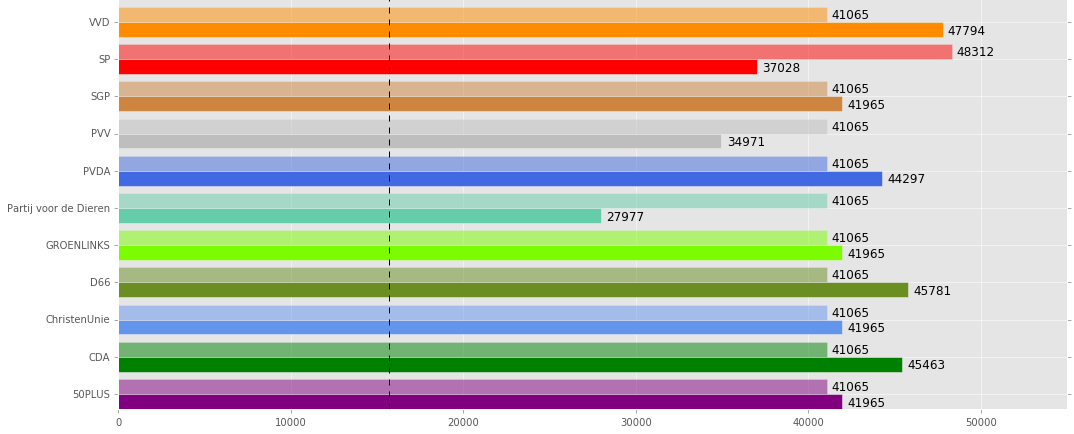
\includegraphics[width=\linewidth]	{stemmen_op_provincialen_topN_samen.png}

			\caption{Grafiek met per partij de verdeling van de stemmen van provinciale kiezers op alle provinciale kandidaten van de partij a.d.h.v. de peiling (licht gekleurd) en a.d.h.v. de einduitslag (donker gekleurd). De stippellijn is de daadwerkelijk voorkeursdrempel(15.708 stemmen).}

\label{fig:stemmenS1P}
\end{figure}


Zoals te zien in Figuur \ref{fig:stemmenS1P} hierboven, zijn zowel volgens de peiling (voorspelling) alsmede volgens de einduitslag alle top \textit{N} provinciale kandidaten van de partijen boven de daadwerkelijke voorkeursdrempel uitgekomen. Ofschoon de precieze aantallen niet exact hetzelfde zijn, is met strategie 2 de voorspelling zoals berekend a.d.h.v. de peiling correct in het voorspellen welke partijen met alle provinciale kandidaten boven de voorkeursdrempel uitkomen en welke partijen dit niet het geval is.

\paragraph{Aantal provincialen na strategie 1.}
Na het uitvoeren van de strategie 1 en het opstellen van de Tweede Kamer zoals eerder in dit hoofdstuk beschreven, levert strategie 1 een Tweede Kamer op waarin  138 provincialen en 12 Randstedeling plaatsnemen. Daarmee zijn provincialen (met 92\%) zeer ruim in hogere mate vertegenwoordigd dan Randstedelingen (met 8\%) . In de cirkeldiagram in Figuur \ref{fig:pcS1P} hieronder is de verdeling goed te zien. 

\begin{figure}[H]
\centering
	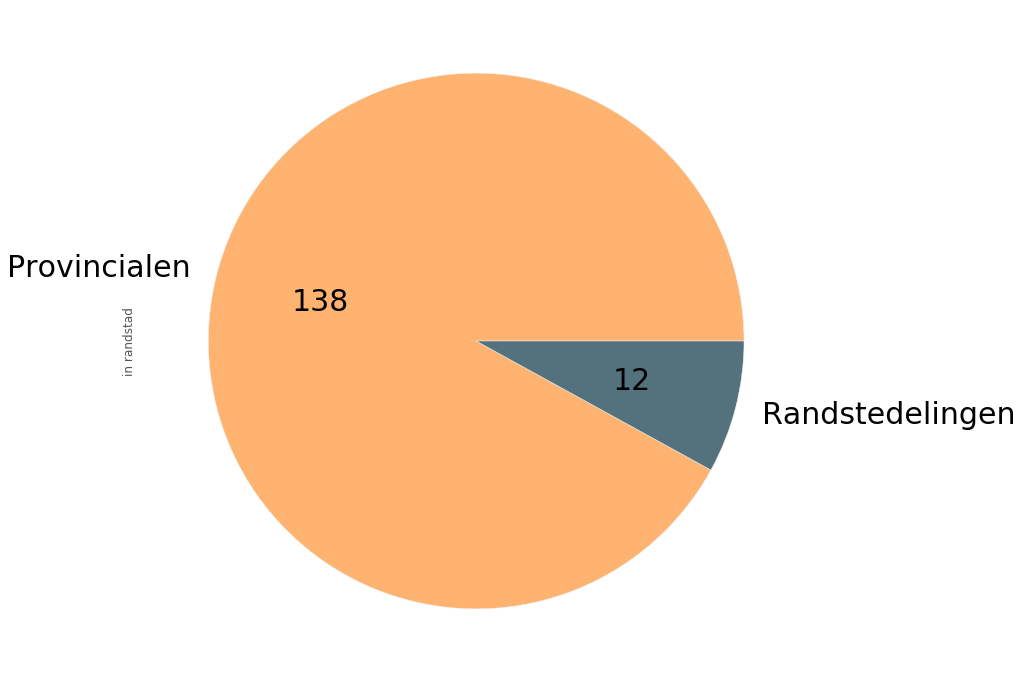
\includegraphics[width=0.45\linewidth]{pie_chart_topN_provincialen.png}

			\caption{Na uitvoering van de strategie nemen er 138 provincialen(92\%) en 12 Randstedelingen(8\%) plaats in de Tweede Kamer.} 

\label{fig:pcS1P}
\end{figure}

\paragraph{Minder dan 147 provincialen in de Tweede Kamer na uitvoering van strategie 1.}
De reden dat er niet 147 ouderen maar 'slechts' 138 provincialen in de Tweede Kamer plaatsnemen na uitvoering van strategie 1 ligt ten grondslag aan een aantal factoren. Bij GROENLINKS had de lijstrekker, in de persoon van Jolande 
Sap, meer stemmen dan de provinciale kandidaten. Hierdoor viel bij GROENLINKS één provinciale kandidaat af. De Partij voor de Dieren had de lijsttrekker, in de persoon van Marianne Thieme, ook meer stemmen dan de provinciale kandidaten. Tevens ontving de Partij voor de Dieren één zetel minder bij de einduitslag dan dat de peiling aangaf. Hierdoor vielen er bij de Partij voor de Dieren twee provinciale kandidaten af. Bij de PVV had de lijsttrekker, in de persoon van Geert Wilders, meer stemmen dan de provinciale kandidaten. Tevens ontving de PVV drie zetels minder bij de einduitslag dan dat de peiling aangaf. Hierdoor vielen er bij de PVV vier provinciale kandidaten af. Bij de SP had de nummer twee op de kandidatenlijst, in de persoon van Renske Leijten, meer stemmen dan de provinciale kandidaten.  Tevens ontving de SP vijf zetels minder bij de einduitslag dan dat de peiling aangaf. Hierdoor vielen er bij de SP drie provinciale kandidaten af. Het aantal provinciale in de Tweede Kamer na uitvoering van strategie 1 komt daarom uit op ($147-9$ = ) 138.







\subsubsection{Strategie 2: Provinciale kiezers stemmen op een willekeurige provinciale kandidaat.}

\paragraph{Het toewijzen van de stemmen aan de provinciale kandidaten op basis van de peiling en de einduitslag.}
Op dezelfde wijze als bij de andere strategie\"{e}n wijzen we de hier de provinciale stemmen toe a.d.h.v. de peiling en a.d.h.v. de einduitslag (voor gedetailleerde uitleg zie \hyperref[S1V]{Strategie 1} in \hyperref[vrouwen]{Bevolkingsgroep: Vrouwen}). In Figuur \ref{fig:stemmenS2P} hieronder is zowel de toewijzing op basis van de peiling alsmede de toewijzing op basis van de einduitslag te zien.


\begin{figure}[H]

	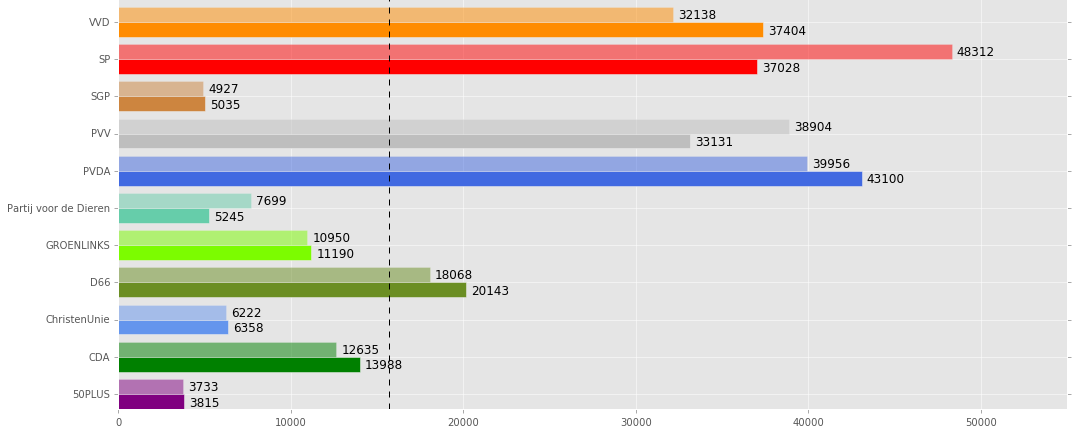
\includegraphics[width=\linewidth]	{stemmen_op_provincialen_willekeurig_samen.png}

			\caption{Grafiek met per partij de verdeling van de stemmen van provinciale kiezers op alle provinciale kandidaten van de partij a.d.h.v. de peiling (licht gekleurd) en a.d.h.v. de einduitslag (donker gekleurd). De stippellijn is de daadwerkelijk voorkeursdrempel(15.708 stemmen).}

\label{fig:stemmenS2P}
\end{figure}

Zoals te zien in Figuur \ref{fig:stemmenS2P} hierboven, zijn zowel volgens de peiling (voorspelling) alsmede volgens de einduitslag niet alle provinciale kandidaten van de partijen boven de daadwerkelijke voorkeursdrempel uitgekomen. Ofschoon de precieze aantallen niet exact hetzelfde zijn, is met strategie 2 de voorspelling zoals berekend a.d.h.v. de peiling correct in het voorspellen welke partijen met alle provinciale kandidaten boven de voorkeursdrempel uitkomen en welke partijen dit niet het geval is. 

\paragraph{Aantal provincialen na strategie 2.}
Na het uitvoeren van de strategie 2 en het opstellen van de Tweede Kamer zoals eerder in dit hoofdstuk beschreven, levert strategie 2 een Tweede Kamer op waarin 127 provincialen en 23 Randstedelingen plaatsnemen. Daarmee zijn provincialen (met  85\%) ruim in hogere mate vertegenwoordigd dan Randstelingen (met 15\%). In de cirkeldiagram in Figuur \ref{fig:pcS2P} hieronder is de verdeling goed te zien. 


\begin{figure}[H]
\centering
	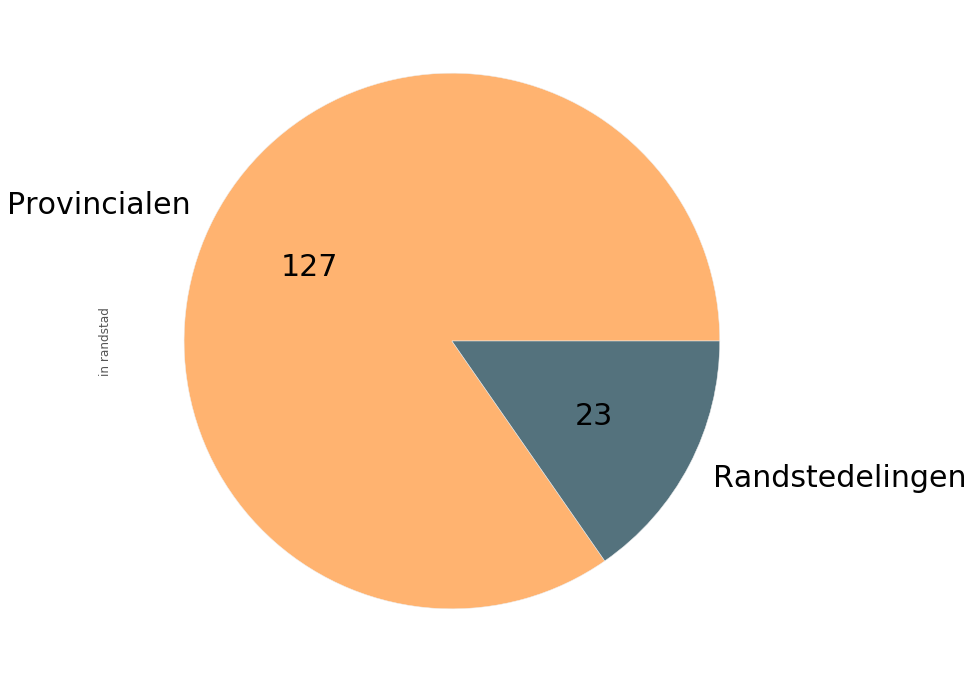
\includegraphics[width=0.45\linewidth]{pie_chart_willekeurig_provincialen.png}

			\caption{Na uitvoering van de strategie nemen er 127 provincialen (85\%) en 23 Randstedelingen (15\%) plaats in de Tweede Kamer.}

\label{fig:pcS2P}
\end{figure}





\paragraph{Elf provincialen minder in de Tweede Kamer ten opzicht van strategie 1.}
De reden dat er niet 138 maar 127 provincialen in de Tweede Kamer plaatsnemen na uitvoering van strategie 2 ligt ten grondslag aan een aantal factoren. Bij het CDA, de ChristenUnie en de SGP hadden de provinciale kandidaten niet genoeg stemmen gekregen om boven de voorkeursdrempel uit te komen. Echter, vanwege de plaats op de kandidatenlijsten, ontvingen vijftien provinciale kandidaten van deze partijen alsnog een zetel. Hierdoor vielen er bij deze partijen echter wel totaal zes provinciale kandidaten af. Bij zowel GROENLINKS alsmede de Partij voor de Dieren hadden de provinciale kandidaten ook niet genoeg stemmen om boven de voorkeursdrempel uit te komen. Tevens ontvingen er bij deze partijen ook geen van de provinciale kandidaten een zetel vanwege het feit dat de zij te laag op de kandidatenlijsten stonden. Hierdoor vielen er bij deze partijen vier provinciale kandidaten af. Bij de PVV hadden zowel de lijsttrekker (Geert Wilders) als de nummer twee op de lijst (Fleur Agema) meer stemmen dan de provinciale kandidaten. Hierdoor viel er bij de PVV één kandidaten af. Geen enkele partij krijgt meer provincialen in de Tweede Kamer na uitvoering van strategie 2 ten opzichte van strategie 1. Het aantal provincialen in de Tweede Kamer na uitvoering van strategie 2 komt daarom uit op ($138-11$ = ) 127.



\subsubsection{Strategie 3.1: Provinciale kiezers stemmen willekeurige op één van de eerste 15 provinciale kandidaten van een partij.}

\paragraph{Partijen met minstens 15 provinciale kandidaten en partijen met minder dan 15 provinciale kandidaten.}
In de grafiek in Figuur \ref{fig:15P} hieronder zien we dat bij alle partijen de provinciale stemmen over de top 15 provinciale kandidaten verdeeld kunnen worden.

\begin{figure}[H]

	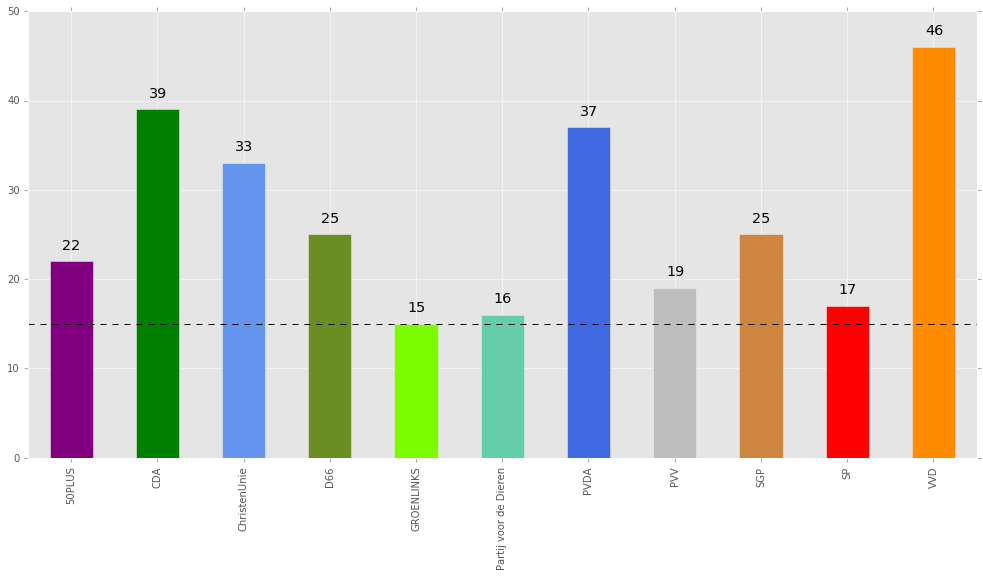
\includegraphics[width=\linewidth]	{top15_of_topN_kandidaten_provincialen.png}

			\caption{De grafiek toont dat bij alle partijen de provinciale kiezers op de top 15 provinciale kandidaten van de partij kunnen gaan stemmen (\textit{N=15}).}

\label{fig:15P}
\end{figure}


\paragraph{Het toewijzen van de stemmen aan de provinciale kandidaten op basis van de peiling en de einduitslag.}
Op dezelfde wijze als bij de andere strategie\"{e}n wijzen we de hier de provinciale stemmen toe a.d.h.v. de peiling en a.d.h.v. de einduistlag (voor gedetailleerde uitleg zie \hyperref[S1V]{Strategie 1} in \hyperref[vrouwen]{Bevolkingsgroep: Vrouwen}). In Figuur \ref{fig:stemmenS31P} hieronder is zowel de toewijzing op basis van de peiling alsmede de toewijzing op basis van de einduitslag te zien.

\begin{figure}[H]

	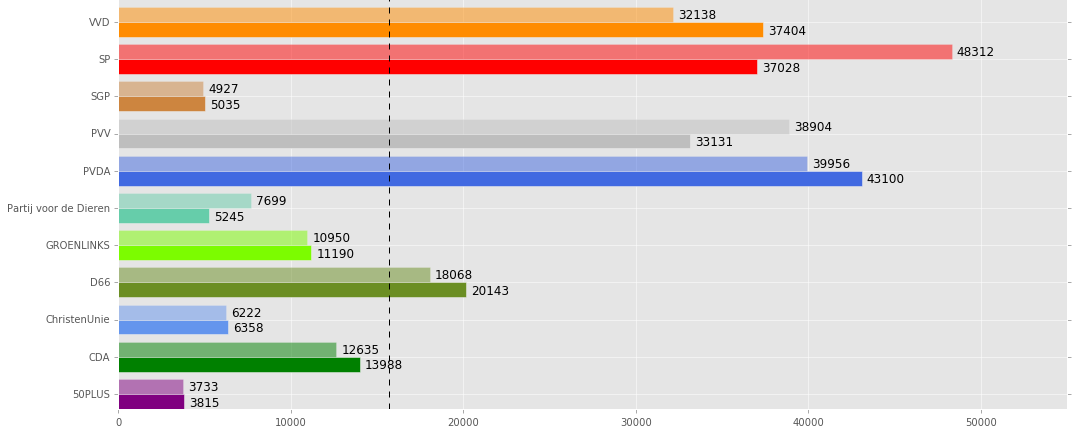
\includegraphics[width=\linewidth]	{stemmen_op_provincialen_top15_of_topN_samen.png}

			\caption{Grafiek met per partij de verdeling van de stemmen van provinciale kiezers op alle provinciale kandidaten van de partij a.d.h.v. de peiling (licht gekleurd) en a.d.h.v. de einduitslag (donker gekleurd). De stippellijn is de daadwerkelijk voorkeursdrempel(15.708 stemmen).}

\label{fig:stemmenS31P}
\end{figure}

Zoals te zien in Figuur \ref{fig:stemmenS31P} hierboven, zijn zowel volgens de peiling (voorspelling) alsmede volgens de einduitslag niet alle provinciale kandidaten van de partijen boven de daadwerkelijke voorkeursdrempel uitgekomen. Ofschoon de precieze aantallen niet exact hetzelfde zijn, is met strategie 3.1 de voorspelling zoals berekend a.d.h.v. de peiling correct in het voorspellen welke partijen met alle provinciale kandidaten boven de voorkeursdrempel uitkomen en welke partijen dit niet het geval is. 

\paragraph{Aantal provincialen na strategie 3.1.}
Na het uitvoeren van de strategie 3.1 en het opstellen van de Tweede Kamer zoals eerder in dit hoofdstuk beschreven, levert strategie 3.1 uiteindelijk een Tweede Kamer op waarin 103 provincialen en 47 Randstedelingen plaatsnemen. Daarmee zijn provincialen (met 69\%) in hogere mate vertegenwoordigd dan Randstedelingen(met 49\%). In de cirkeldiagram in Figuur \ref{fig:pcS31P} hieronder is de verdeling goed te zien. In de volgende paragraaf wordt uitgelegd waarom er niet 127 (zoals in de vorige strategie) maar slechts 103 provincialen in de Tweede Kamer Plaatsnemen na uitvoering van strategie 3.1 ten opzichte van strategie 2.

\begin{figure}[H]
\centering
	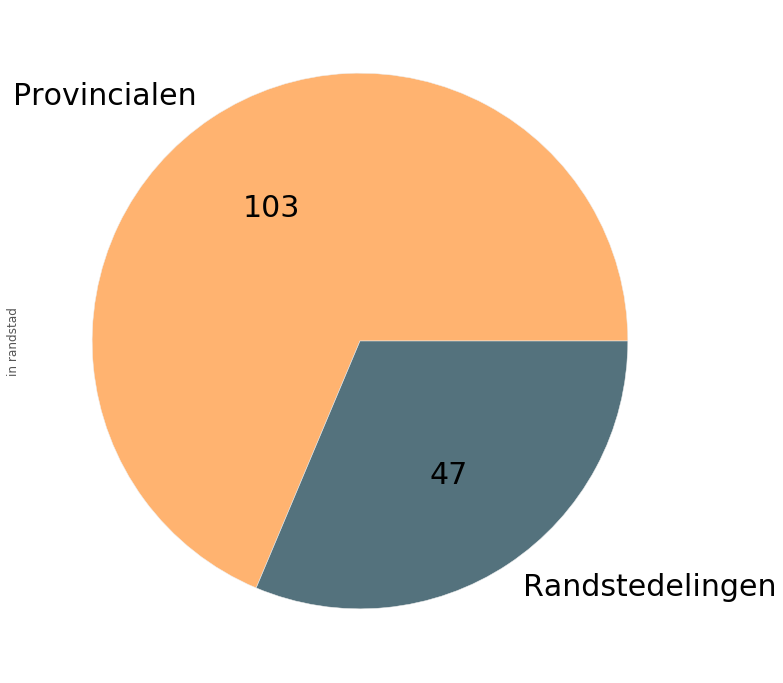
\includegraphics[width=0.4\linewidth]{pie_chart_top15_of_topN_provincialen.png}

			\caption{Na uitvoering van de strategie nemen er 91 vrouwen(61\%) en 59 mannen(39\%) plaats in de Tweede Kamer.}

\label{fig:pcS31P}
\end{figure}

\paragraph{Minder provincialen in de Tweede Kamer d.m.v. uitvoering van strategie 3.1 dan d.m.v. uitvoering van strategie 2.}
De reden dat er, na uitvoering van strategie 3.1, 103 provincialen in de Tweede Kamer plaatsnemen en dat er daarmee 24 provincialen minder plaatsnemen in de Tweede Kamer dan bij strategie 2 het geval zou zijn ligt ten grondslag aan het feit dat er bij de PVDA achttien provinciale kandidaten afvallen ten opzichte van strategie 2. Dit komt omdat de stemmen niet verdeeld worden over alle 37 provinciale kandidaten van de PVDA maar over de top 15 provinciale kandidaten van de PVDA. Drie andere proviniciale kandidaten van de PVDA ontvingen een zetel vanwege hun plaats op de kandidatenlijst. Bij de VVD vielen er elf provinciale kandidaten af. Ook bij de VVD komt dit doordat de stemmen verdeeld worden over de top 15 provinciale kandidaten van de VDD. De overige tien provinciale kandidaten van de VDDontvingen een zetel vanwege hun plaats op de kandidatenlijst. Het CDA, D66 en de PVV kregen ontvingen echter meer zetels. Bij partijen ontvingen de provinciale kandidaten gezamenlijk vijf extra zetels ten opzichte van strategie 2. Daarmee komt het totale aantal provincialen in de Tweede Kamer uit op ($127-24$ = ) 103.



\subsubsection{Strategie 3.2: Provinciale kiezers stemmen willekeurige op één van de eerste \textit{N} provinciale kandidaten van een partij.}


\paragraph{Voor elke partij de eigen \textit{N} bepalen.}
Hieronder is in de grafiek in Figuur \ref{fig:XP} per partij te zien op welke waarde het \textit{N} provinciale kandidaten wordt bepaald. 50PLUS, D66, GROENLINKS, de Partij voor de Dieren, de PVV, de SGP en de SP hebben meer dan vijftien maar minder dan dertig provinciale kandidaten op de kandidatenlijst staan. Voor deze partijen geldt \textit{N=15}. Het CDA, de ChristenUnie, de PVDA en de VVD hebben meer dan dertig provinciale kandidaten op de kandidatenlijst staan. Voor deze partijen geldt \textit{N=30}.

\begin{figure}[H]

	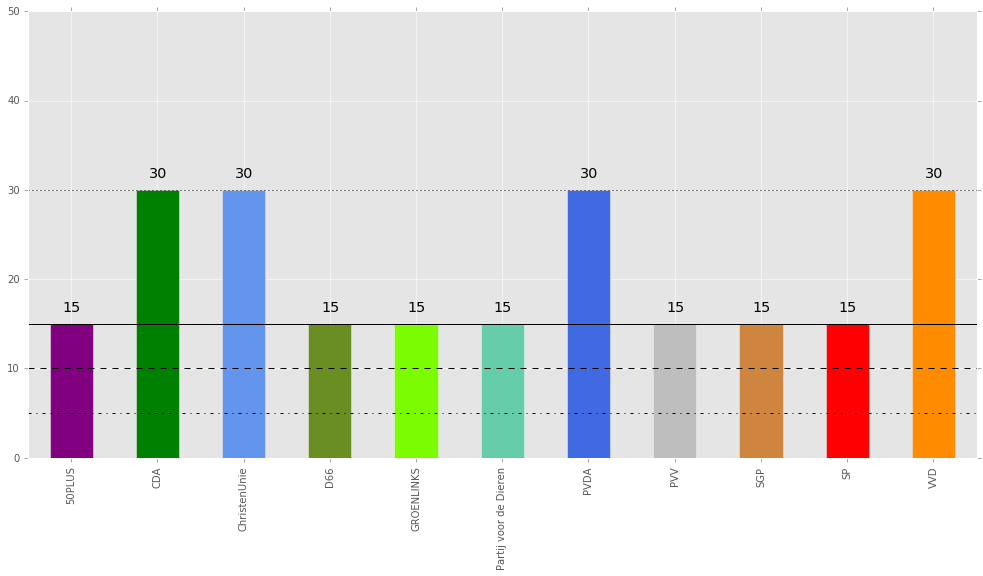
\includegraphics[width=\linewidth]{eigenX_partijen_provincialen.png}

			\caption{Elke partij krijgt een eigen \textit{X}. De lijnen geven een verschillende mogelijk \textit{X} aan.} 

\label{fig:XP}
\end{figure}


\paragraph{Het toewijzen van de stemmen aan de provinciale kandidaten op basis van de peiling en de einduitslag.}
Op dezelfde wijze als bij de andere strategie\"{e}n wijzen we de hier de provinciale stemmen toe a.d.h.v. de peiling en a.d.h.v. de einduitslag (voor gedetailleerde uitleg zie \hyperref[S1V]{Strategie 1} in \hyperref[vrouwen]{Bevolkingsgroep: Vrouwen}). In Figuur \ref{fig:stemmenS32P} hieronder is zowel de toewijzing op basis van de peiling alsmede de toewijzing op basis van de einduitslag te zien.


\begin{figure}[H]

	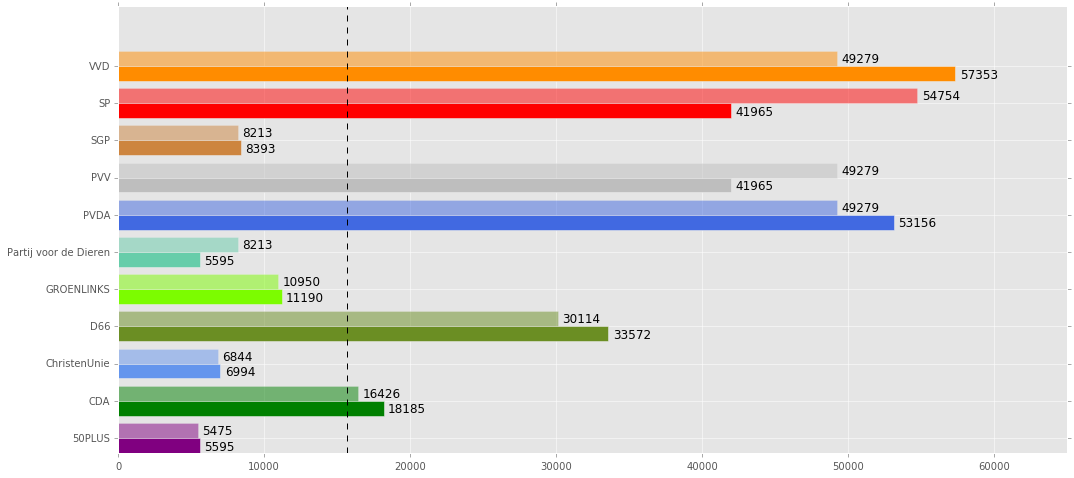
\includegraphics[width=\linewidth]{stemmen_op_provincialen_eigenX_samen.png}

			\caption{Grafiek met per partij de verdeling van de stemmen van provinciale kiezers op alle provinciale kandidaten van de partij a.d.h.v. de peiling (licht gekleurd) en a.d.h.v. de einduitslag (donker gekleurd). De stippellijn is de daadwerkelijk voorkeursdrempel(15.708 stemmen).}

\label{fig:stemmenS32P}
\end{figure}

Zoals te zien in Figuur \ref{fig:stemmenS32P} hierboven, zijn zowel volgens de peiling (voorspelling) alsmede volgens de einduitslag niet alle provinciale kandidaten van de partijen boven de daadwerkelijke voorkeursdrempel uitgekomen. Ofschoon de precieze aantallen niet exact hetzelfde zijn, is met strategie 3.2 de voorspelling zoals berekend a.d.h.v. de peiling correct in het voorspellen welke partijen met alle provinciale kandidaten boven de voorkeursdrempel uitkomen en welke partijen dit niet het geval is.


\paragraph{Aantal provincialen na strategie 3.2.}
Na het uitvoeren van de strategie 3.2 en het opstellen van de Tweede Kamer zoals eerder in dit hoofdstuk beschreven, levert strategie 3.2 een Tweede Kamer op waarin 120 provincialen en 30 Randstedelingen plaatsnemen. Daarmee zijn provincialen (met 80\%) in minder mate vertegenwoordigd dan Randstedelingen (met 20\%). In de cirkeldiagram in Figuur \ref{fig:pcS32P} hieronder is de verdeling goed te zien. In de volgende paragraaf wordt uitgelegd waarom er zeventien provincialen meer in de Tweede Kamer plaatsnemen na uitvoering van strategie 3.2 ten opzicht van strategie 3.1.

\begin{figure}[H]
\centering
	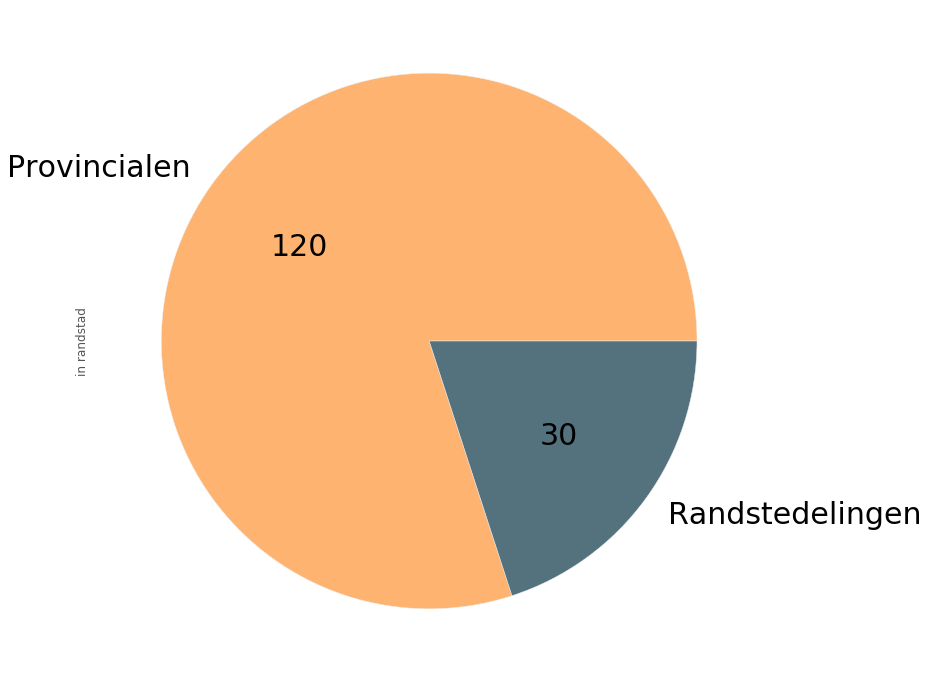
\includegraphics[width=0.45\linewidth]{pie_chart_eigenX_provincialen.png}

\caption{Na uitvoering van de strategie nemen er 120 ouderen(80\%) en 30 Randstedelingen (20\%) plaats in de Tweede Kamer.}

\label{fig:pcS32P}
\end{figure}

\paragraph{Meer provincialen in de Tweede Kamer d.m.v. uitvoering van strategie 3.2 dan d.m.v. uitvoering van strategie 3.1.}
De reden dat er, na uitvoering van stratefie 3.2, 120 provincialen in de Tweede Kamer plaatsnemen en dat er daarmee zeventien provincialen meer zijn ten opzichte van strategie 3.1 ligt ten grondslag aan het feit dat bij de top \textit{N} voor zowel de PVDA alsmede de VVD verandert van \textit{N=15} naar \textit{N=30}. Hierdoor krijgen de PVDA en de VVD respectievelijk dertien en vijf provincialen erbij ten opzichte van strategie 3.1. Bij de overige partijen vallen er geen extra provinciale kandidaten af noch komen er provinciale kandidaten bij. Hierdoor komt het totaal aantal provincialen in de Tweede Kamer op ($103+17$ = ) 120.

\subsubsection{Strategie 4: Provinciale kiezers stemmen op de top \textit{N+extra percentage} provinciale kandidaten van een partij.}
\label{S4P}

\paragraph{Speling in top \textit{N}.}
Zoals te zien in Figuur \ref{fig:zetelsP}, zijn er meerdere partijen die een hoger aantal provinciale kandidaten op de kandidatenlijst hebben staan dan dat verwacht werd dat zij, volgens de peiling, aan zetels zouden gaan ontvangen. Vanwege het feit dat de zetelverdeling volgens de peiling niet 100\% correspondeerde met de zetelverdeling volgens de einduitslag, is het ook voor de bevolkingsgroep provincialen interessant om te kijken wat er gebeurt wanneer de top \textit{N} wordt uitgebreid met een \textit{extra percentage} bovenop de eerder al per partij bepaalde top \textit{N} uit strategie 1.



\paragraph{Maximaal aantal provinciale per partij(top \textit{N+extra percentage}) dat in de Tweede Kamer gekozen kan worden.} 
Bij strategie 4 wordt de top \textit{N} voor elke partij uitgebreid met een \textit{extra percentage} van \textit{N} in stappen van 10\% extra (dus eerst 110\%, dan 120\% etc.). Zodoende worden de provinciale stemmen die een partij ontvangt telkens over de top \textit{N+extra percentage} provinciale kandidaten van de partij verdeeld. Daarbij kan de top \textit{N+extra percentage} van een partij nooit meer worden dat het totaal aantal provinciale kandidaten dat de partij op de kandidatenlijst heeft staan. In Figuur \ref{fig:NexpP} hieronder is er per partij te zien wat er met de top \textit{N} gebeurt wanneer het \textit{extra percentage} hieraan wordt toegevoegd.  


\begin{figure}[H]

	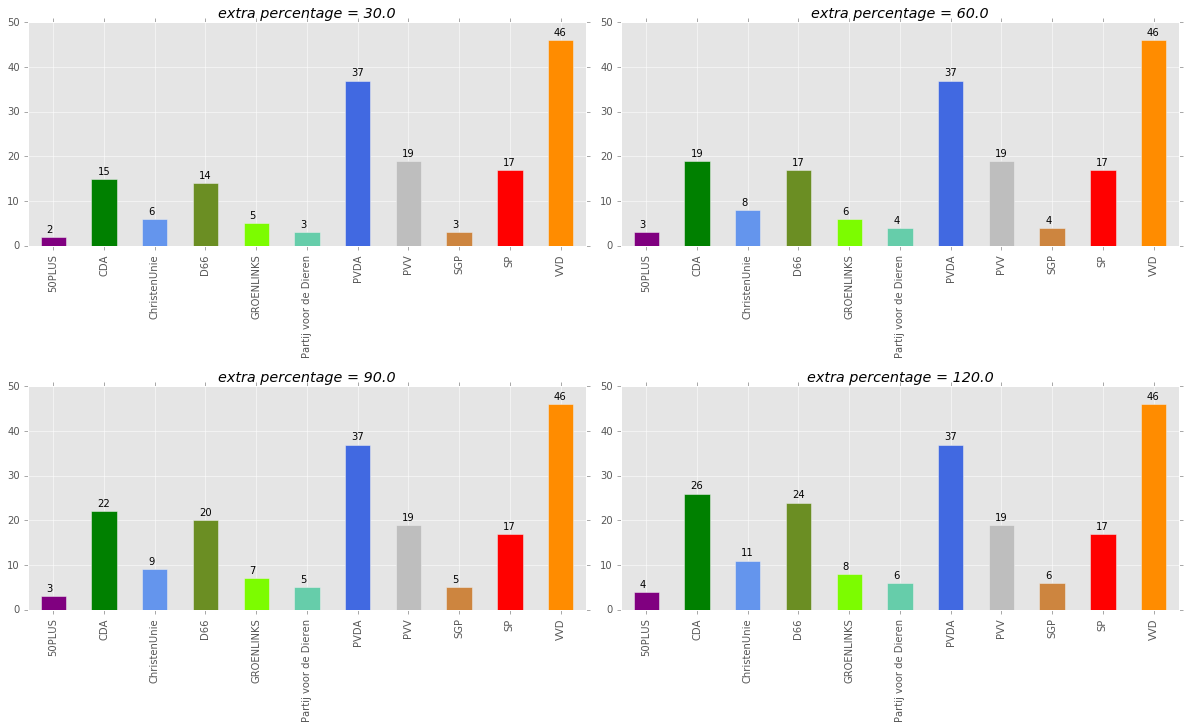
\includegraphics[width=\linewidth]{topN_vermenigvuldiging_provincialen.png}

			\caption{De top \textit{N+extra percentage} waarin \textit{extra percentage} respectievelijk 30\%, 60\%, 90\% en 120\% extra te verwachten zetels (voor provinciale kandidaten) zijn.}

\label{fig:NexpP}
\end{figure}




\paragraph{Het toewijzen van de stemmen aan de provinciale kandidaten op basis van de peiling en de einduitslag.}
Op dezelfde wijze als bij de andere strategie\"{e}n wijzen we de hier de provinciale stemmen toe a.d.h.v. de peiling en a.d.h.v. de einduitslag (voor gedetailleerde uitleg zie \hyperref[S1V]{Strategie 1} in \hyperref[vrouwen]{Bevolkingsgroep: Vrouwen}). In de grafieken in Figuur \ref{fig:stemmenS4P} hieronder is zowel de toewijzing van provinciale stemmen op provinciale kandidaten op basis van de peiling alsmede op basis van de einduitslag voor alle partijen te zien. De toewijzingen worden getoond aan de hand van respectievelijk 30\%, 60\%, 90\% en 120\% (\textit{extra percentage}) extra zetels (voor provinciale kandidaten) waarover de stemmen verdeeld worden.

  
\begin{figure}[H]

	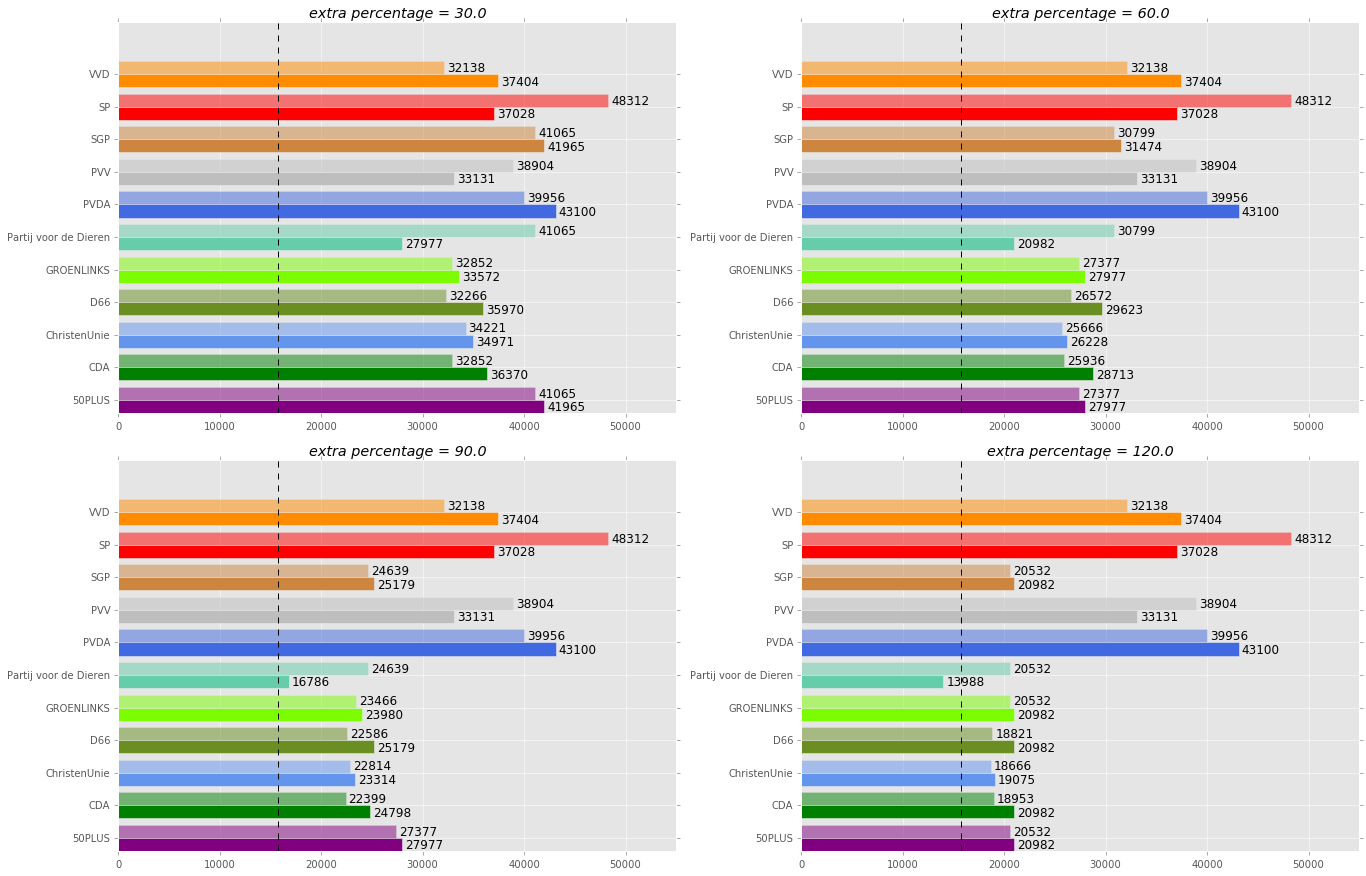
\includegraphics[width=\linewidth]	{stemmen_op_provincialen_topNextrapercentage_uitslag.png}

			\caption{Grafieken in stappen van 30\%, met per partij de verdeling van de stemmen van provinciale kiezers op de top \textit{N+extra percentage} provinciale kandidaten van de partij a.d.h.v. de peiling (licht gekleurd) en a.d.h.v. de einduitslag (donker gekleurd). De stippellijn is de daadwerkelijk voorkeursdrempel(15.708 stemmen).}

\label{fig:stemmenS4P}
\end{figure}

In Figuur \ref{fig:stemmenS4P}  hierboven, is te zien dat zowel volgens de peiling (voorspelling) alsmede volgens de einduitslag bijna alle top \textit{N+extra percentage} provinciale kandidaten van de partijen boven de daadwerkelijke voorkeursdrempel uitkomen wanneer het \textit{extra percentage} aan zetels (voor provinciale kandidaten) wordt verhoogd. Enkel voor de provinciale kandidaten van Partij voor de Dieren blijkt met een \textit{extra percentage=120} bij de einduitslag dat de top \textit{N+ extra percentage} provinciale kandidaten onder de voorkeursdrempel komen. Ofschoon de precieze aantallen niet exact hetzelfde zijn, is met strategie 4 de voorspelling zoals berekend a.d.h.v. de peiling grotendeels correct in het voorspellen welke partijen met de top \textit{N+extra percentage} vrouwelijke kandidaten boven de voorkeursdrempel uitkomen en van welke partijen dit niet het geval is.



\paragraph{Aantal provincialen na strategie 4.}
Na het uitvoeren van strategie 4 en het opstellen van de Tweede Kamer zoals eerder in dit hoofdstuk beschreven, levert strategie 4 bij geen enkel \textit{extra percentage} bovenop de originele \textit{N} uit strategie 1 een hoger aantal provincialen op in de Tweede Kamer. In de grafiek hieronder in Figuur\ref{fig:bcS4P} is te zien hoeveel provincialen er in de Tweede Kamer een zetels bedeeld krijgen wanneer er een bepaald \textit{extra percentage} wordt toegevoegd aan de originele \textit{N} uit strategie 1.

\begin{figure}[H]

	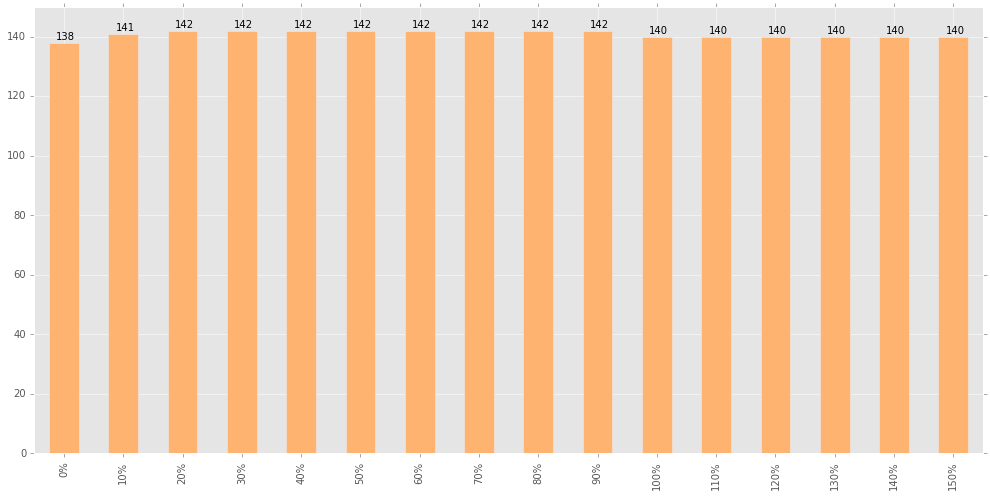
\includegraphics[width=\linewidth]	{topNextrapercentage_aantal_provincialen_overzicht.png}

			\caption{Grafiek met per het aantal provincialen in de Tweede Kamer na uitvoering(en) van strategie 4 in stappen van 10\% aan \textit{extra percentage} (van \textit{N}) bovenop de \textit{N} uit strategie 1.}

\label{fig:bcS4P}
\end{figure}

\paragraph{Niet meer provincialen na uitvoering van strategie 4.}
Zoals hierboven in Figuur \ref{fig:bcS4P}  te zien, komen er na uitvoering van strategie 4 en het toenemen van het \textit{extra percentage} bij extra percentage van 10\% boven de \textit{N} uit strategie 1 al drie provincialen meer in de Tweede Kamer dan bij strategie 1. Bij 20\% extra percentage bovenop de \textit{N} uit strategie 1, komen er zelfs vier extra provincialen in de Tweede Kamer. Dit gaat zo door totdat het aantal provincialen in de Tweede Kamer tussen \textit{extra percentage=90} en \textit{extra percentage=100}, bovenop de \textit{N} uit strategie 1, weer omlaag gaat. Zodoende is strategie 4 bij de provincialen voor het eerst succesvol in het uitbreiden van het aantal vertegenwoordigden van een bevolkingsgroep uit strategie 1.


\paragraph{Niet meer dan 142 provincialen in de Tweede Kamer.}
De reden dat er meer dan 138 provincialen uit strategie 1 maar niet meer dan 142 provincialen in de Tweede Kamer plaatsnemen na uitvoering van strategie 4 ligt ten grondslag aan een aantal factoren. Willen er meer provincialen in de Tweede Kamer plaatsnemen dan na uitvoering van strategie 1 dan is het noodzakelijk dat de partijen ook meer zetels kregen bedeeld bij de einduitslag dan dat volgens te peiling was te verwachten. 
\\
\indent Zo ontving bij de einduitslag de VVD maar liefst vijf zetels meer dan dat er volgens de peiling werden verwacht. Hierdoor komen er bij een bepaalde \textit{extra percentage} (om precies te zijn bij \textit{extra percentage=12}) vier zetels voor provincialen van de VVD bij. D66 ontving bij de einduitslag één zetel meer dan volgens de peiling werd verwacht. Hierdoor komt ook bij D66 bij een bepaalde \textit{extra percentage} (om precies te zijn bij \textit{extra percentage=10}) een extra zetel voor de provincialen bij. Bij de PVV echter, viel er bij een bepaalde \textit{extra percentage} (om precies te zijn bij \textit{extra percentage=6}) een provinciale kandidaat af ten faveure van Fleur Agema. Dit omdat Fleur Agema vanaf dat \textit{extra percentage} meer stemmen had dan de provinciale kandidaten van de PVV. Zodoende komt het maximale aantal provinciale in de Tweede Kamer na uitvoering(en) van strategie 4 uit op ($138+4$ = ) 142.


